\documentclass[a4paper,11pt]{article}
\usepackage[utf8]{inputenc}
\usepackage{dmasproject}
% if you need additional LaTeX packages, add them here
\usepackage[T1]{fontenc}
\usepackage{newpxtext,newpxmath}
% \usepackage[left=1in, right=1in, top=1.25in, bottom=1.25in]{geometry}
\usepackage{hyperref}
\usepackage{titling}

% \usepackage{caption}
\usepackage{amsmath}
\usepackage{mathtools}
\usepackage{amsfonts}
\usepackage{amssymb}
\label{mathrefs}

\usepackage{graphicx}
\usepackage{multirow}
\usepackage{pdflscape}

\begin{document}

%% BEGIN TITLE
\begin{titlingpage}
    \begin{center}
    
        % Heading
        {\Huge\bfseries\scshape%
            Glasses for the Visually Impaired \\[0.5em]
        }
        {\Large\bfseries\scshape%
            GENE 403 Design Project Report
        }

        \vspace{5em}
        
        % Authors
        \begin{tabular}{cccc}
            Waleed Ahmed & Martin Ethier & Zain Denno & Connor Barker \\
            ECE & MME & ECE & ECE \\
            20659541 & 20660931 & 20654316 & 20711394 \\
            w29ahmed & methier & zdenno & cpbarker
        \end{tabular}
        
        \vspace{5em}
        
        \tableofcontents
    \end{center}
\end{titlingpage}
%% END TITLE

\newpage

\section{Introduction}
The latest global estimates found that about 253 million people are visually impaired. Of those people, about 36 million are blind, meaning they have little to no vision \cite{orbis-global-blind-data}. Looking specifically at Canada and the United States, an estimated 1.5 million Canadians identify themselves as having sight loss \cite{cnib-blind-data}, and about 7.6 million Americans have a visual disability \cite{nfb-blind-data}. The Vision Loss Expert Group predicts that without increased access to eye health services, these numbers could potentially triple by 2050 \cite{orbis-global-blind-data}.

\

\noindent
Taking a step back, it is worth investigating what being visually impaired or blind actually means. In one of our focus interviews, we were told by somebody who self-identified as blind that "Blindness is a spectrum". Very few people who identify as visually impaired or blind have no light perception at all. For most, blindness is a gradual degradation of sight. Some can see well, but only in certain light conditions. Others can only identify shapes or colours, and some have a field of vision so diverse and complex that is difficult to explain \cite{lighthouse-sf-info-page}. Another diverse aspect of blindness is when it is experienced in life. Some individuals are blind from birth, while others develop it at various points in life. While there are many causes of blindness, the leading ones are cataracts, age-related macular degeneration, glaucoma, diabetic retinopathy, corneal opacity, and trachoma \cite{WHO-blindness}.

\

\noindent
Despite the diversity of conditions and visual impairment out there, there are many common problems faced by this demographic. One of the biggest ones, and a core focus of our project, is reading text. It doesn't occur to sighted individuals just how much text there is out in the world that contains crucial information we rely on to go about our day. Many visually impaired folk do not have this luxury and are missing out on key information that can help them to live more independently. While one solution to this is to ensure accompanying braille text wherever possible, there are still many situations where braille is not available. For example, text on a storefront or a postcard with your name and address on it to let you know the mail is for you.

\

\noindent
Our design solution is to take advantage of cutting-edge advancements in artificial intelligence and computer vision to extract, decode, and communicate text from an image to a visually impaired user through audio transcription. More specifically, we are designing a mobile application and a wearable device (glasses) that will enable the ability to conveniently and efficiently accomplish this task. Some design solutions already exist to accomplish our proposed primary function, and they are described in the need analysis summary (Section \ref{need-analysis-summary}).

\

\noindent
This report summarizes the need analysis, research, verification, development, and project management carried out in the Spring 2021 term as a part of GENE 403 for our initial low fidelity prototype.

\subsection{Key Terminology}

\setlength{\tabcolsep}{1em}
\begin{table}[ht]
    \centering
    \begin{tabular}{|p{5cm}|p{10cm}|}
        \hline
        Optical Character Recognition (OCR) & Broad term that describes any system that can extract and decode text from a digital representation such as an image or PDF \\ \hline
        VoiceOver & Screen reader built into iOS \\ \hline
    \end{tabular}
\end{table}

\newpage
\section{Need Analysis Summary}
\label{need-analysis-summary}

\subsection{Problem Identification}
Since none of the group members are visually impaired, it was important to us to perform need analysis through speaking with individuals who are visually impaired or organizations that represent them. Doing this provided us with useful insight into some of the problems faced by the visually impaired, and allowed us to zero in on the features that would be the most useful to include in our design solution. Through our own research along with recommendations from our faculty advisor, Professor John Zelek, we identified a few organizations that advocate and aid the visually impaired that would be insightful to connect with. We were fortunate enough to hear back and have a chance to speak with a representative from Lighthouse SF and the University of Waterloo's AccessAbility Services.

\subsubsection{Interview with Lighthouse SF}
Lighthouse SF is an organization founded in 1902 and currently has headquarters in San Francisco, California. Their goal is to promote the independence, equality, and self-reliance of people who are blind or have low vision \cite{lighthouse-sf-homepage}. They pool together resources, hold seminars, and offer courses to help people with visual disabilities learn to use the latest and greatest assistive technologies. The individual that we had a chat with is currently an assistive technology instructor at the organization and self-identified herself as being blind.

\

\noindent
During the interview, we discussed the various assistive technologies that exist and what her experience was with using them. She also enumerated a few very specific use cases where OCR technology currently does well, and where there is room for improvement. Some key takeaways were:

\begin{itemize}
    \item In the context of reading a physical book, one useful feature would be if the technology can automatically detect when the page has been turned and start reading out the next page without any additional explicit input from the user.
    \item There are two widely used "visual interpreter" apps called Be My Eyes and Aira. These apps connect the user with a sighted individual through a video call to assist in a task. The key difference between the two apps is that Be My Eyes works through sighted volunteers who lend their time for free and do not require any professional training, while Aira employs agents that are professionally trained visual interpreters to respond to calls.
    \item In the context of OCR, she mentioned that the most useful feature amongst other apps was the ability to instantly read out the text from a video feed, and in the cases where an image needs to be captured, audio-guided camera capture was useful. An example of audio-guided capture is when you are trying to get a picture of a document, all 4 corners of the document need to be visible for the image processing pipeline to extract out just the document from the image. One app, in particular, will say things like "left corner not visible" to inform the user why the captured image was not sufficient.
    \item One of the complaints about current OCR technology is that it does not perform well on handwritten text or non-standard machine fonts.
    \item She gave us a great quote: "Blindness is a spectrum" when we asked about the usability of wearable glasses. She mentioned that due to the diversity amongst visually impaired folks, some might know how to put on and use glasses due to losing their sight later in life, but it might not be as intuitive to someone who has been blind since birth.
    \item Another feature we asked her about is above the waist obstacle detection using computer vision. She mentioned that this is a feature that is not present in many solutions, but warned us that it is not as useful of a feature as we might think. It is only applicable in few scenarios, many individuals already use a white cane that is cheap and very capable for obstacle detection/avoidance in most scenarios.
    \item She informed us of a monthly meetup called Lighthouse Labs where engineers and developers working on assistive technology for low vision come to present their ideas. She extended an invite for us to attend and showcase what we end up building.
\end{itemize}

\noindent
Overall, our biggest takeaway from the interview with Lighthouse SF was to double down on OCR as the primary feature of our design, as we spent the most time talking about it and we got the impression that it is the feature that is most useful. While we do have other additional features in mind, such as depth estimation, scene description, and money detection, we don't plan on spending any time on those until we feel confident our OCR works well.

\subsubsection{Interview with UW AccessAbility Services}
AccessAbility Services is responsible for working with students with disabilities to develop personalized academic accommodations at the University of Waterloo \cite{uw-accessability}. We spoke with a representative from the office who was employed as an adaptive educational technologist. There are 3 functional areas the office focuses on: class, assignments, and tests. Examples of potential services provided within the context of a visually impaired student for each of the functional areas are:
\begin{itemize}
    \item Class
    \begin{itemize}
        \item Reserved seating in a classroom if a student wishes to sit closer to the front or back
        \item Request professors to provide a transcript of lecture slides
        \item Request professor to allow student to audio or video record the lectures so that they can listen and transcribe them later on their own
        \item Note-taking services, such as asking for student volunteers to provide notes
        \item Get a textbook translated into braille or audio format
    \end{itemize}
    
    \item Assignments
    \begin{itemize}
        \item Asking for extensions to accommodate for additional difficulties of learning the content with a disability
    \end{itemize}
    
    \item Tests
    \begin{itemize}
        \item Getting students a scribe
        \item Requesting for oral tests instead of written tests
        \item Exams are done in special test centres where computers are setup that can read out the text for each question
        \item Get a test translated into braille
    \end{itemize}
\end{itemize}

\newpage
\noindent
In addition, a few technologies/products were mentioned that students had used in the past, including:
\begin{itemize}
    \item Jaws: Screen reading technology for the Windows operating system \cite{jaws-software}
    \item Kurzweil 3000: Educational software with text to speech features \cite{kurzweil}, not specifically tailored for visually impaired users though
    \item Read\&Write by TextHelp: A literary support tool that has useful OCR features in it \cite{read-and-write}. However, similar to Kurzweil, it's targeted at a general audience, in particular, grade school students
    \item Speechify: Mobile and desktop app for those with reading difficulties, low vision, and anybody interested in converting reading material to an audio format. Can read anything from the web, PDF, or images \cite{speechify}
\end{itemize}

\noindent
There are even more assistive technologies available, and a more comprehensive list along with tutorials on how to use them are available on learn by self-registering for AccessAbility Services, which is available for every student, regardless of whether or not they are registered with a disability.

\

\noindent
When asked what some of the complaints students had about existing technologies, we were told that screen reading technology often gets thrown off by weird formatting (captions, footnotes, etc.), and sometimes the voice reading it out can be a bit robotic. Speechify was highlighted as having realistic voices that are more pleasant and engaging to listen to.

\

\noindent
Our key takeaway from this interview was an overview of some of the difficulties faced by visually impaired students in the context of academics. We were also pointed towards a lot of currently available products and technologies that are adjacent to our proposed design solution. Additionally, we mentioned if it would be possible for us to send out a survey or request to speak with visually impaired students to provide us with informal discussion/feedback on our design solution. We were told this is something that could be organized if we wish to proceed, and we plan on exploring this avenue later on in our design process in order to conduct some user studies and testing on our design.


\subsection{Survey of Available Products/Technologies}
Many products and solutions already exist in our chosen problem space. Reviewing them closely and identifying the pros and cons of each one allowed us to focus on the things that could be done better and potentially addressed by our solution. The five products we choose to focus on are Orcam MyEye 2, Envision, Seeing AI, Speechify, and Be My Eyes. Others exist, but these five are the closest and most relevant to our proposed design solution, so they are most valuable to examine.

\subsubsection{OrCam MyEye 2}
The OrCam MyEye 2 \cite{orcam} is a piece of hardware that can be attached magnetically to an existing pair of glasses. It is designed specifically for blind and visually impaired users and has a wide array of features to support that demographic. It can be controlled by voice or touch and can accomplish tasks such as read text, recognize faces, identify products, recognize barcodes, recognize money, and identify colours. Best of all, it can do all these features offline, meaning a network connection is not required. This means all of the processing is done right on the glasses. When we first identified the problem space and thought of potential solutions, something like the OrCam MyEye 2 is precisely what we originally had in mind. However, what we quickly realized with this product and others like it is that they are very expensive. Pricing information isn't readily available without consultation with OrCam, but we did find an article \cite{orcam-price} that mentioned \$3500 USD. Additionally, OrCam listed it on Amazon for \$5800 CAD \cite{orcam-amazon}. Even though the exact pricing isn't clear, it seems that the cost for this device is multiple thousands of dollars, which is very high. Globally, there are an estimated 200 million people who do not have access to assistive products for low vision \cite{WHO-assistive}. One of the reasons for this is products can be very expensive, and some individuals with a visual impairment may not have sufficient financial resources to purchase products with a premium price tag.

\

\noindent
While the technology in this product is cutting edge and very useful, we feel that with some design changes, primarily offloading compute to a server or a user's phone, it should be possible to deliver a similar feature set at a much more accessible price point. After examining the OrCam MyEye, we identified cost as our primary constraint and focused on finding a solution that can minimize it.

\subsubsection{Envision}
Envision has two products, an app and a pair of glasses, targeted for the visually impaired \cite{envision}. The app can be used on its own without the glasses, and it uses the phone's camera instead of a camera attached to glasses. The app has features for reading text, scene description, colour detection, barcodes, and configurable object and people detection. The app initially comes with a one-week free trial, and then afterward runs on a subscription model. As of August 7th, 2021, the prices in CAD for the app are below:
\begin{center}
    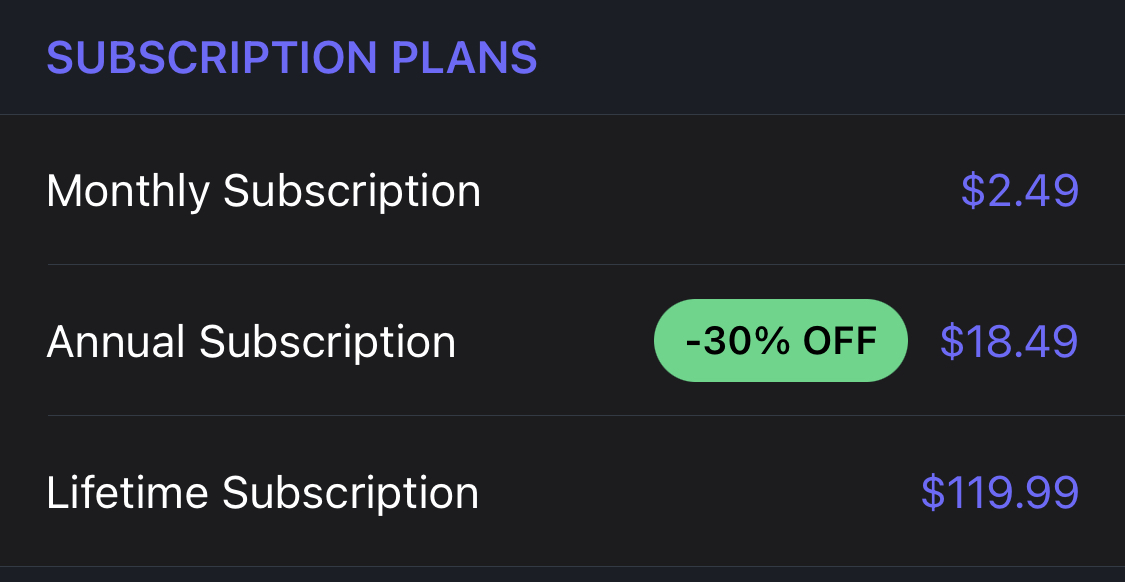
\includegraphics[width={0.7\linewidth}]{img/envision_app_price.jpeg}
\end{center}

\noindent
Envision also has a pair of wearable glasses, built on top of the Google Glasses platform. All the features on the app are accessible with the glasses as well, as well as one additional feature that enables a video call that broadcasts a direct feed from the glasses. It is not clear from their website which of these features can run offline and which ones run online, as the glasses are capable of both wifi and Bluetooth. It's obvious that the video calling feature would require a network connection, but text detection could be done both offline or online. Additionally, the purchase of the glasses comes with a lifetime subscription to the accompanying application for both iOS and Android.

\ 

\noindent
Similar to the OrCam MyEye, Envision is a great product with some cutting-edge features that are undeniably very useful for the visually impaired demographic. However, it suffers a similar problem in that it is very expensive. As of August 8th, 2021, the base model for Envision is listed as 3268.91 pounds, which is 5696.87 CAD.

\newpage
\subsubsection{Seeing AI}
Seeing AI is a free application on iOS built as a part of Microsoft's "AI for Good" initiative \cite{seeing-ai}. Seeing AI has a lot of the same features that OrCam MyEye and Envision have, such as real-time short text detection, document reading, barcodes, face recognition, scene description, currency detection, and color detection. Two features that Seeing AI has that we couldn't confirm if MyEye or Envision have is handwritten text detection and light detection. Light detection is a unique feature that plays a sound that indicates how much light the camera detects. 

\

\noindent
Some of these features work offline using on-device processing, while others utilize Microsoft's Azure cloud services and require a network connection. The features that require a network connection are document scanning, face detection, scene description, and handwritten text. The rest work offline.

\ 

\noindent
The amazing part about this application is that it is totally free. There is no subscription or additional features available at a price. We found various other applications on the app store that would do a subset of features offered by Seeing AI, but they were not free. As a result, Seeing AI is considered the gold standard application for the visually impaired, as it is totally free and has a rich feature set. The individual we spoke to from Lighthouse SF was very familiar with this app and reported using it regularly.

\

\noindent
After trying out this application, we really started to question if making a pair of glasses is even the way to go. If the end goal is to make it as cheap and accessible as possible, it's hard to compete with a free app that can do so much. The key insight that made us realize an affordable pair of glasses is still worthwhile to develop is the fact that it can be used without having to pull out and unlock your phone. Let's consider a specific example of wanting to read the name on a postcard. With Seeing AI, you'd have to pull out your phone, unlock it, find and open the Seeing AI app, switch to the "instant text" mode, and then have it read out the text for you. This might not seem so bad, but this process can be cumbersome for somebody who is visually impaired. However, with our solution, it would only require you to look towards the text you are trying to read, press a button on the glasses, and then after a small wait, the text will be read to you. This is fewer steps and allows you to more quickly read text out in the world. With this insight, we decided to continue pursuing our proposed design solution, even knowing now that a free alternative does exist.

\subsubsection{Speechify}
Speechify is a desktop and mobile app that can turn various forms of text into audio \cite{speechify}. The app is built on the premise that listening to something is easier and faster than reading it. It is not specifically for any demographic, but it can be used by anyone who has reading difficulty due to things like ADHD, Dyslexia, or visual impairment. Many people who have no problem reading still use Speechify, as it can increase productivity to get through large pieces of text faster by listening to it at faster speeds. Speechify can read anything on the internet, files, or images. It comes with a free option but there are paid features available, such as different voices that sound less robotic. This app was brought to our attention by UW AccessAbility services, as one of the complaints of many OCR technologies is the voice sounds very robotic, and Speechify was praised for having options for more realistic voices.

\newpage
\subsubsection{Be My Eyes}
Be My Eyes is a free app that allows blind and visually impaired people to connect with sighted volunteers through a video call \cite{be-my-eyes}. This allows a sighted individual to assist in a task that a visually impaired person is having trouble with. Signing up to be a volunteer is free, and Connor has been a volunteer on the app for some time and has picked up three calls in the past. Waleed signed up for the app early in the term but has yet to get a notification to pick up a call. We examined this app as a way to potentially have interactions with visually impaired people, and get some insight into the kind of tasks that they need assistance with. An example use case would be for navigating an outdoor park. A visually impaired user may be in search of a bench to sit at and is not sure where to go. They can place a call for assistance on the app and a sighted volunteer will pick up and through the mobile phone's camera, guide the user to a nearby bench to sit at.

\

\noindent
A notable mention is another app called Aira, which is built on the same premise as Be My Eyes, but instead of connecting visually impaired users with sighted volunteers, Aira employs trained visual interpreters who pick up the call.

\

\noindent
Internally, we had some discussion about enabling a video call through the camera on the glasses, similar to the Envision glasses. This is not a high priority for us at the moment, but due to the success and usefulness of services such as Be My Eyes and Aira, it is something we are open to investigating further if time permits.

\subsubsection{Summary and Key Takeaways}
Assistive devices for the visually impaired is a problem space that has existed for quite some time, and as such, many solutions and products are currently available. Products like the OrCam MyEye 2, Envision, and Seeing AI offer a rich feature set and try to cover as many use cases as possible. The common feature, and the first one that each solution talks about, is the ability to detect and read text using OCR technology. It is reasonable to conclude that this is the most useful feature present in these solutions, and likely the one that gets the most usage. Therefore, we are choosing to focus on OCR as our primary feature, and only once we have that down will we start to consider some of the other features.

\ 

\noindent
Additionally, due to the existence of Seeing AI, we plan on focusing our user experience around the glasses as much as possible. While we do want our app to eventually work without the glasses as well, and the user can simply use their phone's camera, it is less important to us since this functionality is already covered and implemented very well by Seeing AI. Our goal is to push this problem space forward with something that isn't too similar with what already exists.


\newpage
\subsection{Patent Surveys}
The breadth of existing products with the same functionality as our solution has required us to carefully consider patent law when planning the design of our project. Specifically, OrCam owns a variety of patents protecting both their hardware and software products \cite{orcam-patents}. As the MyEye 2 is the device that most closely resembles our solution, we used their patent list as a starting point for our research. Other products, such as EnVision and NuEyes, possess IP as well, although these patents are either pending \cite{envision-patent} or unrelated to our solution.

\

\noindent
Conveniently, the reason OrCam products are so expensive is also the reason we can successfully avoid patent infringement in our design. OrCam's patents are entirely related to proprietary software \cite{orcam-software} and hardware \cite{orcam-hardware}. Because we are using prefabricated hardware in the form of the Raspberry Pi and existing machine-learning software frameworks, neither of these components infringes upon OrCam's patents. OrCam does have some specific patents related to using a wearable camera in combination with machine learning software to drive an assistive device, although crucially these patents universally discuss performing machine learning on-platform. By offloading our machine-learning inference tasks to another device (the iPhone and servers), rather than using a dedicated processing device, our solution exists outside of the intellectual property patented by OrCam.

\

\noindent
There is a possible issue of patent infringement concerning the doctrine of equivalents \cite{doctrine-of-equivalents}. This doctrine is a common legal rule which states that a device that does not literally fall within the realm of a patent may still be infringing upon said patent if it performs an identical function. This principle is often a legal grey area, and disputes regarding it are typically settled through a patent lawyer. While not experts, we believe that our solution avoids the doctrine of equivalents. While the system as a whole does perform a similar function to the OrCam MyEye 2, the subsystems involved do not. The wearable hardware's only purpose is to transmit an image wirelessly to either a server or a paired mobile app. In turn, the mobile application/server's only responsibility is to perform optical character recognition on an image. This image can be transmitted from an external source, or possibly captured by the smartphone camera. As a result, the solution performs an arguably different function entirely to OrCam's product. One of the qualifiers for the doctrine of equivalents to come into effect is that a "person skilled in the art" should consider the device or process equivalent to the patent being infringed upon \cite{doctrine-of-equivalents}. We feel confident that the novel addition of performing machine-learning on a mobile device and servers significantly differentiates our solution from OrCam's.

\newpage
\section{Design Solution Summary}
\noindent
The design consists of three interacting components: a wearable device attached to a pair of glasses, the user's iOS device, and a cloud server. The glasses are the user's main point of interaction and include a button that kicks off a processing pipeline to complete Optical Character Recognition (OCR) on the scene at which the user's head is pointed. The glasses are connected to the server using a WiFi network, and to the iOS device using a Bluetooth Low Energy (BLE) connection. The server is used to perform OCR processing, and the iOS device is used to perform text to speech and audio playback of the final result. An iOS application will be used to guide a user through using the device and setting preferences.

\

\noindent
There are two text modalities the design will be aimed at: machine text, and text "in the wild". Machine text refers to digitally generated text on relatively flat surfaces, i.e. books, documents, screens, e-readers. Text in the wild is a larger category that includes any text that may be seen on a day-to-day basis. This can range anywhere from logos and packaging to signs. The latter modality presents unique challenges in that the text may come in non-standard fonts and colours, and may be printed on surfaces that aren't flat. We had also considered supporting handwritten text as a third modality, but after consulting scientific literature and currently available open-source libraries, we concluded that current state-of-the-art models won't generalize well enough to real-world handwritten text examples for it to be useful.

\

\noindent
Please see section \ref{section-system-level} for a system-level representation and a more detailed description of the design solution.

\newpage
\section{Design Verification/Validation Summary}
\subsection{Review of Compliance to Engineering Design Specification}
See section \ref{eds-0.2} for the latest version of our engineering design specification. Below is a table with status estimates and comments on progress for each specification.

\

\noindent
\textbf{General}
\begin{table}[ht]
    \centering
    \begin{tabular}{|p{0.7cm}|p{1cm}|p{10cm}|}
    % \begin{tabular}{|c|c|c|}
        \hline
        No. & Status (\%) & Comments \\ \hline
        
        1.1 & 20 & Validated some features, but yet to bring it all together into a low fidelity prototype. \\ \hline
        
        1.2 & 100 & Current hardware is well below price target. \\ \hline
        
        1.3 & 100 & Connecting Raspberry Pi Zero W to Wifi is straightforward and we have validated it works. \\ \hline
        
        1.4 & 20 & Have done some preliminary research and testing using Bluetooth on the Raspberry Pi. Have yet to try pairing and using it with an iOS application. \\ \hline
        
        1.5 & 100 & We are assuming this to always be true in our design. We can alert the user if the iOS device is not nearby and a Bluetooth connection can no longer be established. \\ \hline
    \end{tabular}
\end{table}

\noindent
\textbf{Software - General}
\begin{table}[ht]
    \centering
    \begin{tabular}{|p{0.7cm}|p{1cm}|p{10cm}|}
    % \begin{tabular}{|c|c|c|}
        \hline
        No. & Status (\%) & Comments \\ \hline
        
        2.1.1 & 20 & Done preliminary design for UI/UX for both iOS application and hardware interface. Have yet to test and use VoiceOver with our solution. \\ \hline
        
        2.1.2 & 0 & Inclusion of the server was only recently added to the EDS. Have yet to do any preliminary research into available platforms and their usual uptimes. If we go with an established service like AWS or Google Cloud this requirement should not be difficult to accomplish. \\ \hline
    \end{tabular}
\end{table}

\noindent
\textbf{Software - iOS}
\begin{table}[ht]
    \centering
    \begin{tabular}{|p{0.7cm}|p{1cm}|p{10cm}|}
    % \begin{tabular}{|c|c|c|}
        \hline
        No. & Status (\%) & Comments \\ \hline
        
        2.2.1 & 10 & Similar to specification 1.4, done some preliminary testing on Bluetooth, but yet to try integrating it with an iOS app. \\ \hline
        
        2.2.2 & 5 & Have not tried using BLE yet, only researched it to verify it is possible to use it for background processing. \\ \hline
        
        2.2.3 & 40 & Have tested and validated speech to text is possible on iOS, but have not tried to run it in background. \\ \hline
    \end{tabular}
\end{table}

\newpage
\noindent
\textbf{Software - Artificial Intelligence}
\begin{table}[ht]
    \centering
    \begin{tabular}{|p{0.7cm}|p{1cm}|p{10cm}|}
    % \begin{tabular}{|c|c|c|}
        \hline
        No. & Status (\%) & Comments \\ \hline
        
        2.3.1 & 25 & Machine text is handled well by most models we tested. Have not tried it out on a custom test but it is likely this requirement won't be difficult to meet. \\ \hline
        
        2.3.2 & 10 & Text in the wild is a bit harder. Have tried OCR models on text in the wild, and some models have done well while others haven't. EasyOCR is the most promising, but have yet to build a custom test set and check it's F-score on that. \\ \hline
        
        2.3.3 & 0 & Not focusing on this yet as we haven't finalized which models we are going to use. Haven't thought yet about how we will convey this to user. \\ \hline
    \end{tabular}
\end{table}

\noindent
\textbf{Hardware}
\begin{table}[ht]
    \centering
    \begin{tabular}{|p{0.7cm}|p{1cm}|p{10cm}|}
    % \begin{tabular}{|c|c|c|}
        \hline
        No. & Status (\%) & Comments \\ \hline
        
        3.1 & 0 & Have not tried connecting GPIO to Raspberry Pi Zero W yet. We do have access to hardware buttons for testing though. \\ \hline
        
        3.2 & 0 & Have not tried connecting GPIO to Raspberry Pi Zero W yet. We do have access to a piezoelectric buzzer for testing though. \\ \hline
        
        3.3 & 100 & Raspberry Pi Zero W has a 5V port. Well understood requirement. Easy and quick to verify. \\ \hline
        
        3.4 & 70 & Very intense workload draw around 230mA, so we expect to meet this requirement with ease. We will be employing a USB tester to monitor the current draw as the design develops. \\ \hline
        
        3.5 & 100 & Piezoelectric speakers are well understood and well documented. Will be easy to test. \\ \hline
        
        3.6 & 50 & Using documentation, we expect to meet this requirement. Easy to test, but not verifiable until the design is complete and can operate at a realistic workload. \\ \hline

    \end{tabular}
\end{table}

\newpage
\noindent
\textbf{Safety \& Regulatory}
\begin{table}[ht]
    \centering
    \begin{tabular}{|p{0.7cm}|p{1cm}|p{10cm}|}
    % \begin{tabular}{|c|c|c|}
        \hline
        No. & Status (\%) & Comments \\ \hline
        
        4.1 & 70 & Easily verified. USB cables/ports are well designed and relatively safe. Packaging will be designed to make the design safe even further. \\ \hline
        
        4.2 & 0 & Have not implemented error detection in the design. Once implemented, will be easy to test. \\ \hline
        
        4.3 & 0 & Requirement is highly related to packaging, and all progress has been focused on technical implementation so far. \\ \hline

    \end{tabular}
\end{table}


\section{Design for Safety}
\noindent
There are several facets of safety we are considering when designing and implementing our solution. For one, as with any electronic device, it is essential that our design does not present any electrical harm to the user. Since the design is an assistive device for the visually impaired, we will also be taking action to try to avoid putting the user in harm's way.

\subsection{Safety of Electrical Components}
\noindent
There are several considerations to be made to ensure that no potentially harmful electrical components are exposed. The key area of concern is the micro USB power port that will be used to connect to the battery. We will be using packaging to cover as much of the port as possible. Additionally, the current draw of the Raspberry Pi Zero W using a USB digital current meter as described in Section \ref{elec-verification} in Appendix B.

\subsection{Safety in Use}
\noindent
We aim to implement error detection and feedback such that the user can always stay informed on the status of the device. We will be employing the following feedback mechanisms to achieve our safety goal:
\begin{itemize}
    \item \textbf{Model Confidence}: OCR models provide results alongside a measure of confidence. This metric will be communicated to the user to keep them more aware of the performance of the system.
    \item \textbf{Piezoelectric Buzzer}: To be used to play a tone to the user informing them of errors in the system, e.g. connection to phone lost, connection to WiFi lost, etc.
    \item \textbf{Orientation Feedback}: It is not outside the realm of possibility for a user to place an item or sign in a position where a portion of the text is cut off. In such a case, we aim to detect when the text is difficult to read and instruct the user on how to remedy the situation.
    \item \textbf{Haptic Actuators}: Our "bucket list" of features includes navigation assistance. In the case that this goal becomes achievable within the scope of the Capstone timeline, we will use haptic actuators to assist in communicating direction information and hazard proximity.
\end{itemize}
The above feedback options, when integrated with the system, will allow the device to not put the user in a position of relying on the device if it's unable to perform as best as it can.

\newpage
\section{Design for Regularity Requirements}
\noindent
Ontario (and the Canadian government), like many legal jurisdictions around the world, has regulations regarding the manufacture and sale of assistive devices. However, these regulations primarily impose restrictions upon medical technology. Our solution is non-intrusive and does not attempt or promise to perform a medical function of any kind. It, therefore, does not meet the requirements to be categorized as even a Class I medical device.

\

\noindent
While our solution may not need to adhere to laws governing medically assistive devices, there are other regulations relating to data usage and privacy that must be carefully considered. The primary feature of the device is to read text to the user from a written or printed source, including medical paperwork, letters, and other sensitive or personal documentation. Data ownership in Canada is governed by an overlapping set of provincial and federal regulations, which apply differently to various use cases \cite{pipeda}. Our solution does not store any data, nor does it tie images taken by the user to them in any way. As such, the device is compliant with all relevant regulations.


\newpage
\section{Design for Sustainability}
\noindent
Our project has two primary components, being the wearable hardware platform and the accompanying mobile application. Additionally, the application and/or hardware may communicate with a cloud platform or similar server solution. Each of these constituent components has its own requirements when designing for sustainability, which must be equally considered in the final design.

\

\noindent
The solution's hardware has the most obvious sustainability issues, as it uses a PCB, battery, and camera. All of these components are difficult to recycle as they consist of a number of small, intricate pieces, each of which is composed of a different material (e.g. the camera has several lenses, an integrated PCB with copper fittings and capacitors, etc). E-waste disposal is becoming a more common problem, and as such, systems for properly disposing of or recycling these parts do exist \cite{ewaste}. We plan to take advantage of them by keeping the hardware as modular as possible. By using a Raspberry Pi instead of a custom PCB, we increase the ease with which the processor can be recycled. The Raspberry Pi Zero is a mass-produced component, meaning that it can be disposed of along with other Raspberry Pis from different sources. The battery is easy to detach, being connected to the Pi via a universal micro-USB cable. Similarly, the camera module connects to the Pi using a standardized ribbon cable. Collectively, this means that the three main components which make up the electronic hardware can be separated and properly disposed of without the use of specialized tools or knowledge. Once the internals have been removed, the housing can be recycled as any other plastic would be.

\

\noindent
The mobile application which performs the majority of the solution's processing has its own set of sustainability requirements, although it also has features that inherently support waste prevention. By offloading the machine learning inference tasks to an iPhone, we can take advantage of the device's highly optimized hardware to perform image recognition quickly and without consuming a large amount of power. This drastically lowers the energy consumption of our solution, and the efficient nature of the iPhone's machine learning acceleration hardware means that running repeated model inference shouldn't have a negative impact on the overall life of the user's phone battery \cite{neural-efficiency}. This solution has the added benefit of not generating additional e-waste. A user will already have an iPhone, meaning that not only do they provide the hardware used by our solution, but the phone can be recycled using Apple's iPhone disposal program at the end of its lifespan \cite{iphone-recycle}. Additionally, it's important to note that performing machine learning inference on separate devices means that the battery required to power the Raspberry Pi and accompanying camera can be much smaller, as the Pi itself only has to compress and send a photo, rather than running a neural network.

\

\noindent
Finally, any potential server component needs to be analyzed for efficiency. Because we wouldn't be constructing or maintaining servers ourselves, the only way to improve sustainability is to reduce the storage and energy consumed by the code we have running in the cloud. By maximizing the efficiency of our server application, we in turn minimize the cycles taken to perform a given task, ultimately reducing the energy consumption of the system. We can further decrease the power requirements by not storing photos uploaded to the server. By keeping data transient, we minimize the storage needed in order to run the application. This could be accomplished by using an AWS Lambda function rather than keeping a server constantly running. Lambda functions only run when they are called, as compared to an always-on server which consumes resources when idling.

\newpage
\section{Impact on Society and Environment}
\noindent
It is an unfortunate fact that despite increasing awareness and regulatory support, many disabilities are not accommodated in day-to-day life. This can force an individual with a disability to ask for help when performing a mundane task, or worse yet be unable to do it at all. In our preliminary analysis, we found that one of the universal needs of the disabled is independence. This is also the most significant way in which our solution impacts society at large.


\

\noindent
The entire premise of our solution is increasing the independence of the blind or partially sighted when interacting with systems that are not designed to support accessibility (i.e. written materials without an accompanying braille translation). The solution is also designed to not be intrusive or obvious; almost all users of the product will have access to a pair of headphones, as iPhones come packaged with wired earbuds. The device is designed not to draw significant attention to the user, as smart glasses (while still not especially prevalent) are an established concept, and our product is functionally indistinguishable from them upon initial inspection. This low-profile, accessibility-improving solution fills an important niche for the blind or visually impaired when going about their lives with as much independence as possible.

\

\noindent
As previously mentioned in our survey of available technologies, products that are functionally similar to our solution do exist. However, they are prohibitively expensive, particularly for disabled individuals who may be on a fixed income or have limited ability to work. The inexpensive nature of our solution makes it drastically more accessible to those who need it, increasing its potential to improve the independence of the disabled. It is our opinion that products designed to improve accessibility should adhere to that principle in all aspects of their design, including affordability for the groups they target.

\

\noindent
Furthermore, we intend to make the entire platform (software, hardware, accompanying instructions) fully open-source. We firmly believe that the benefits of making the solution publicly available far outweigh any downsides related to losing profit should our project become a fully-fledged product. Not only does this make the product even more inclusive to those on a limited budget, but it provides the opportunity for technologically-minded individuals who are blind or partially sighted to contribute valuable new ideas and features we may not have considered. This has the added benefit of increasing the independence of the community as a whole; rather than needing to rely on general-purpose products which may not perfectly suit the requirements of an individual, open-sourcing the project means that a user can easily modify their own system, or build a new one based on our design.

\newpage
\section{Design Project Management Summary}
\subsection{Design Project Plan Changes}
Our project plan and schedule have gone through a few iterations throughout the term. The reason for this is that when we initially planned the project, we made a few technical assumptions that were yet to be tested or validated. The discovery of technology limitations and a survey of available products forced us to rethink the direction of our project a few times. We anticipate this can still happen, as there are still some things we have yet to validate, but we feel more optimistic about our current project plan and believe it is feasible.

\

\noindent
Our biggest technical blockers have been the use of the iOS platform to do some of our processing. Since the iOS development ecosystem is exclusively controlled by Apple, they have many guidelines and limitations on how it can be used. For example, the Bluetooth Low Energy (BLE) data rate is very limited in order to preserve battery life and we realized it is not sufficient to send an image in a reasonable amount of time. This forced us to rethink our project and drop the requirement of it being able to run offline, as we have to rely on a network connection to enable higher data transfer rates to communicate images to a backend server for processing instead of a mobile phone.

\

\noindent
Currently, we only plan on using the iOS device to perform speech synthesis, which means taking a block of text and converting it to audio. This allows us to avoid having to deal with audio hardware on the glasses, and we can rely on the infrastructure available on iOS to play the audio on the phone or to Bluetooth-connected headphones.

\ 

\noindent
Please refer to Section \ref{appendix-c}: Appendix C for the original and current schedule.

\subsection{Management Lessons Learned}
For most of us, this is our first time planning and working on a project that is intended to last longer than a few months. As such, we are bound to make some mistakes in the process, but we also did some things that have worked well.

\

\noindent
One of the things we did well was to agree to meet weekly for internal meetings and biweekly with our faculty advisor. This gave us a minimum of one sync point every week where we could update each other on progress and make sure to bring any blockers to attention quickly. We also ensured to take weekly meeting logs so we had a record of what was discussed and worked on each week. See Section \ref{meeting-logs} for an overview of our meeting log setup. Our communication as a team is strong, as we are very transparent and not afraid to challenge each other's ideas in a constructive manner. Any time there was a disagreement on how to progress, we were able to talk it out and converge on an approach that everybody agreed with. We intend to continue our meeting cadence both internally and with our faculty advisor going forward for Fall 2021 and Winter 2022.

\

\noindent
One of the things we did not do well was assigning timelines and due dates on tasks. We took a very free-flowing approach to tasks, where we didn't decide on a deliverable date to aim for, and left it up as a discretion to the person working on it when it could be done by. As a result, there was a lack of accountability and some tasks dragged on for a very long time. Our plan to mitigate this is to start using ClickUp as our project management software. All tasks are added to ClickUp with an assignee along with a due date, and we intend to review the ClickUp Gantt charts at every internal meeting. This will ensure we have a visual representation of progress at all times, and we can update due dates and timelines accordingly if tasks are taking longer than expected. The due dates on each task will give each member some accountability of when to try and have things done. Please refer to Section \ref{current-timeline} to see a current snapshot of our ClickUp workspace.

\section{Conclusions and Next Steps}
A bulk of this term was spent on problem identification, need analysis, research, and preliminary validation of the individual components of our design. We went through some major iterations and potential design changes, mainly due to technical constraints becoming apparent to us. This trend is likely to continue, as we start to try out and validate more of our proposed features, and we are open to our design going through more iterations. Our hope is that, in the end, we can build a useful prototype and present a feasible product plan to bring a cheap and effective visual aid solution to market.

\

\noindent
In Fall 2021, three of our team members will be on a co-op term. As a result of this, the team will have significantly more free time to dedicate to prototyping and working on this project. We aim to make significant technical progress and come into Winter 2022 with a prototype that is very close to being finished. If everything goes according to plan, we will have a working prototype with capable OCR functionality, and the Winter 2022 term will be spent refining, adding additional features, and preparing for the final capstone deliverables.


% \section{Recommendations for Future Work}

\section{Acknowledgements}
Thank you to the individuals from Lighthouse SF and UW AccessAbility Services (not named for anonymity) who took the time and effort to speak to our team. Their insights and connection will be useful throughout the development process, and we intend to touch base with them again in the future. Thank you as well to our faculty advisor, Professor John Zelek, for meeting with us on a biweekly basis to discuss progress and provide valuable technical consultation. Finally, a thank you to Professor Oscar Nespoli for his useful design knowledge presented in the GENE 403 course content.

\newpage
\section{Appendix A - Design Solution Description}
\subsection{System Level Representation}
\label{section-system-level}

\begin{figure}[H]
\centering
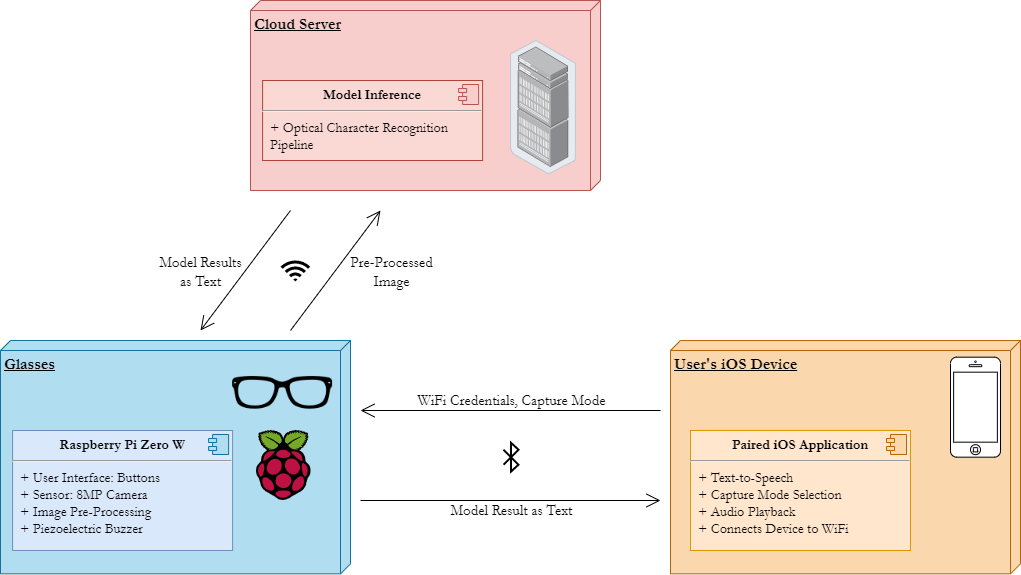
\includegraphics[scale=0.45]{img/System Level.png}
\caption{System Level Design Representation}
\label{fig:system_level}
\end{figure}

\noindent
As shown in figure \ref{fig:system_level}, our design solution consists of three active components: a wearable device in the form of glasses, the user's iOS device, and a cloud server. The glasses will be the main point of interaction for a user.

\

\noindent
The glasses will be equipped with a hardware platform consisting of a Raspberry Pi Zero W \cite{rpi-zero-w}, a 8-megapixel camera \cite{rpi-camera}, some buttons for user interaction, and a piezoelectric buzzer to play sounds to indicate processing and error states.


\

\noindent
A button on the glasses will be used to trigger the computation pipeline. The camera will be used to capture an image of the scene at which the user's head is pointed. The system will take advantage of the processor available on-board the Raspberry Pi Zero W in order to lightly process the image by scaling down its dimensions and converting the image's colour space to grayscale, greatly reducing the size of the image and lessening the data cost and latency of transferring it to the server.

\

\noindent
The server will be used to run an Optical Character Recognition (OCR) pipeline to extract meaningful text data from the image captured by the device, returning the results as text. The ideal case is for this stage of computation to be completed on the iOS device, but this requires Bluetooth modes inaccessible to devices without MFi certification from Apple \cite{apple-mfi}. MFi certification is a process wherein certified devices are able to use an authentication chip that allows them to use connection modes and protocols normally inaccessible. This process is not open to us, as we are not a firm designing a commercial product. However, if we were to pursue this design in a scaled manufacturing capacity, we would certainly seek MFi certification in hopes of eliminating the need for a server altogether. Without a server, we would be able to decrease the overall cost of the design, as well as possibly remove the need for WiFi as a communication medium. 


% Additionally, MFi certification is also needed to access Wireless Accessory Configuration (WAC) entitlement from Apple \cite{apple-wac}, which allows a third party device to receive WiFi credentials from an iOS device. As a result of this constraint, it won't be possible for us to configure the glasses properly from the iOS application, and we will have to manually configure the network configuration everytime on the Raspberry Pi Zero W.

\

\noindent
The user's iOS device will be used to relay the results of the OCR engine by employing a text-to-speech engine, most likely just using Apple's native speech synthesis libraries \cite{apple-speech-synthesis}. The text will be sent from the glasses to the iOS device using Bluetooth Low Energy (BLE). Additionally, we are aiming to do the text to speech processing along with audio playback while the iOS device is locked. This will ensure the user does not need to have the iOS device out and in their hand. This is an important design goal as some blind and visually impaired people use a white cane for navigation, so one hand will already be occupied with that, leaving only one hand left to interact with our design. If the user has to have their iOS device out and open, the user experience will be very poor. We have yet to fully validate if the processing and playback can be done while the iOS device is locked. It is possible to run background tasks on iOS initiated by devices that are Bluetooth Low Energy (BLE) enabled, but we have yet to try it out for ourselves. This is currently the biggest technical risk in our design, and we plan on spending early Fall 2021 to validate this functionality.

\

\noindent
The iOS application may also be used to send WiFi credentials to the on-glasses device. This feature is inaccessible to us without MFi certification, as it is required to gain Wireless Accessory Configuration (WAC) entitlement from Apple \cite{apple-wac}, which allows a third-party device to receive WiFi credentials from an iOS device. As a result of this constraint, it won't be possible for us to configure the glasses properly from the iOS application, and we will have to manually configure the network connection every time on the Raspberry Pi Zero W. As mentioned already, if we were to pursue this design in a scaled manufacturing capacity, we would seek MFi certification to get past this constraint and enable a better user experience.

\

\noindent
An example use of this system would go as follows:
\begin{enumerate}
    \item User presses a button on the eyeglasses device.
    \item Device captures a photo of the user's point of view.
    \item Device scales the photo and transforms it to grayscale to prepare for transfer.
    \item Device pings the cloud server and transfers the image over WiFi.
    \item Server runs the OCR pipeline on the image.
    \item Server returns the results of the computation in text form, it is received by the device over WiFi.
    \item Device pings the user's iOS device and forwards the results of the OCR pipeline using Bluetooth Low Energy (BLE).
    \item iOS device performs speech synthesis to convert text to audio and plays it through the iOS device's audio output (speakers or Bluetooth connected headphones).
\end{enumerate}

% We have plans of attempting to stream video from the glasses to allow for integration with apps like Be My Eyes \cite{be-my-eyes}, that allow visually impaired users to connect with volunteers to help them complete some complicated tasks. After our research with people involved in technologies aimed at the visually impaired, allowing the camera feed from the glasses device to be used with Be My Eyes could prove to be an extremely useful feature to a user.


% \newpage

\begin{landscape}
    \subsection{Engineering Design Specification}
    \subsubsection{v0.1}
    \begin{center}
        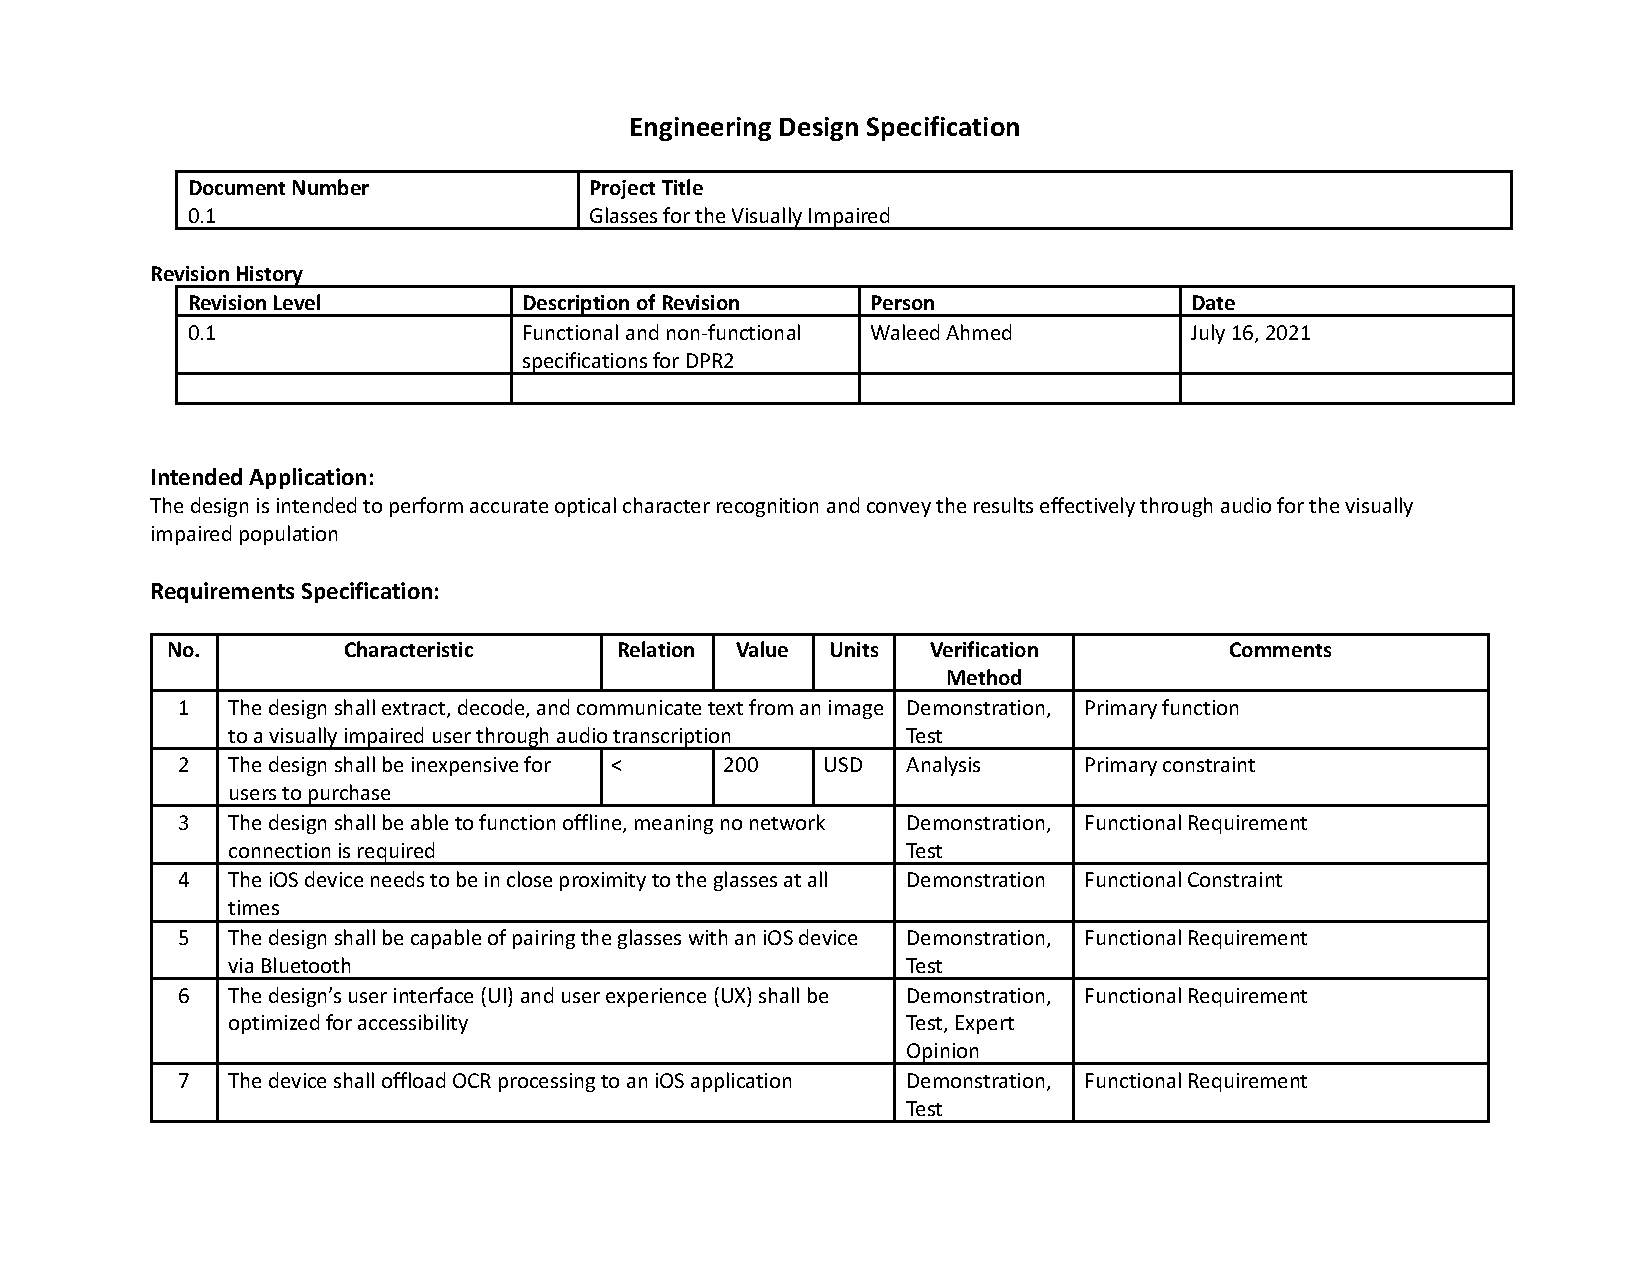
\includegraphics[page=1,width={0.86\linewidth}]{pdf/eds_0.1.pdf}
        \newpage
        \includegraphics[page=2,width={0.86\linewidth}]{pdf/eds_0.1.pdf}
    \end{center}
    
    \newpage
    \subsubsection{v0.2}
    \label{eds-0.2}
    \begin{center}
        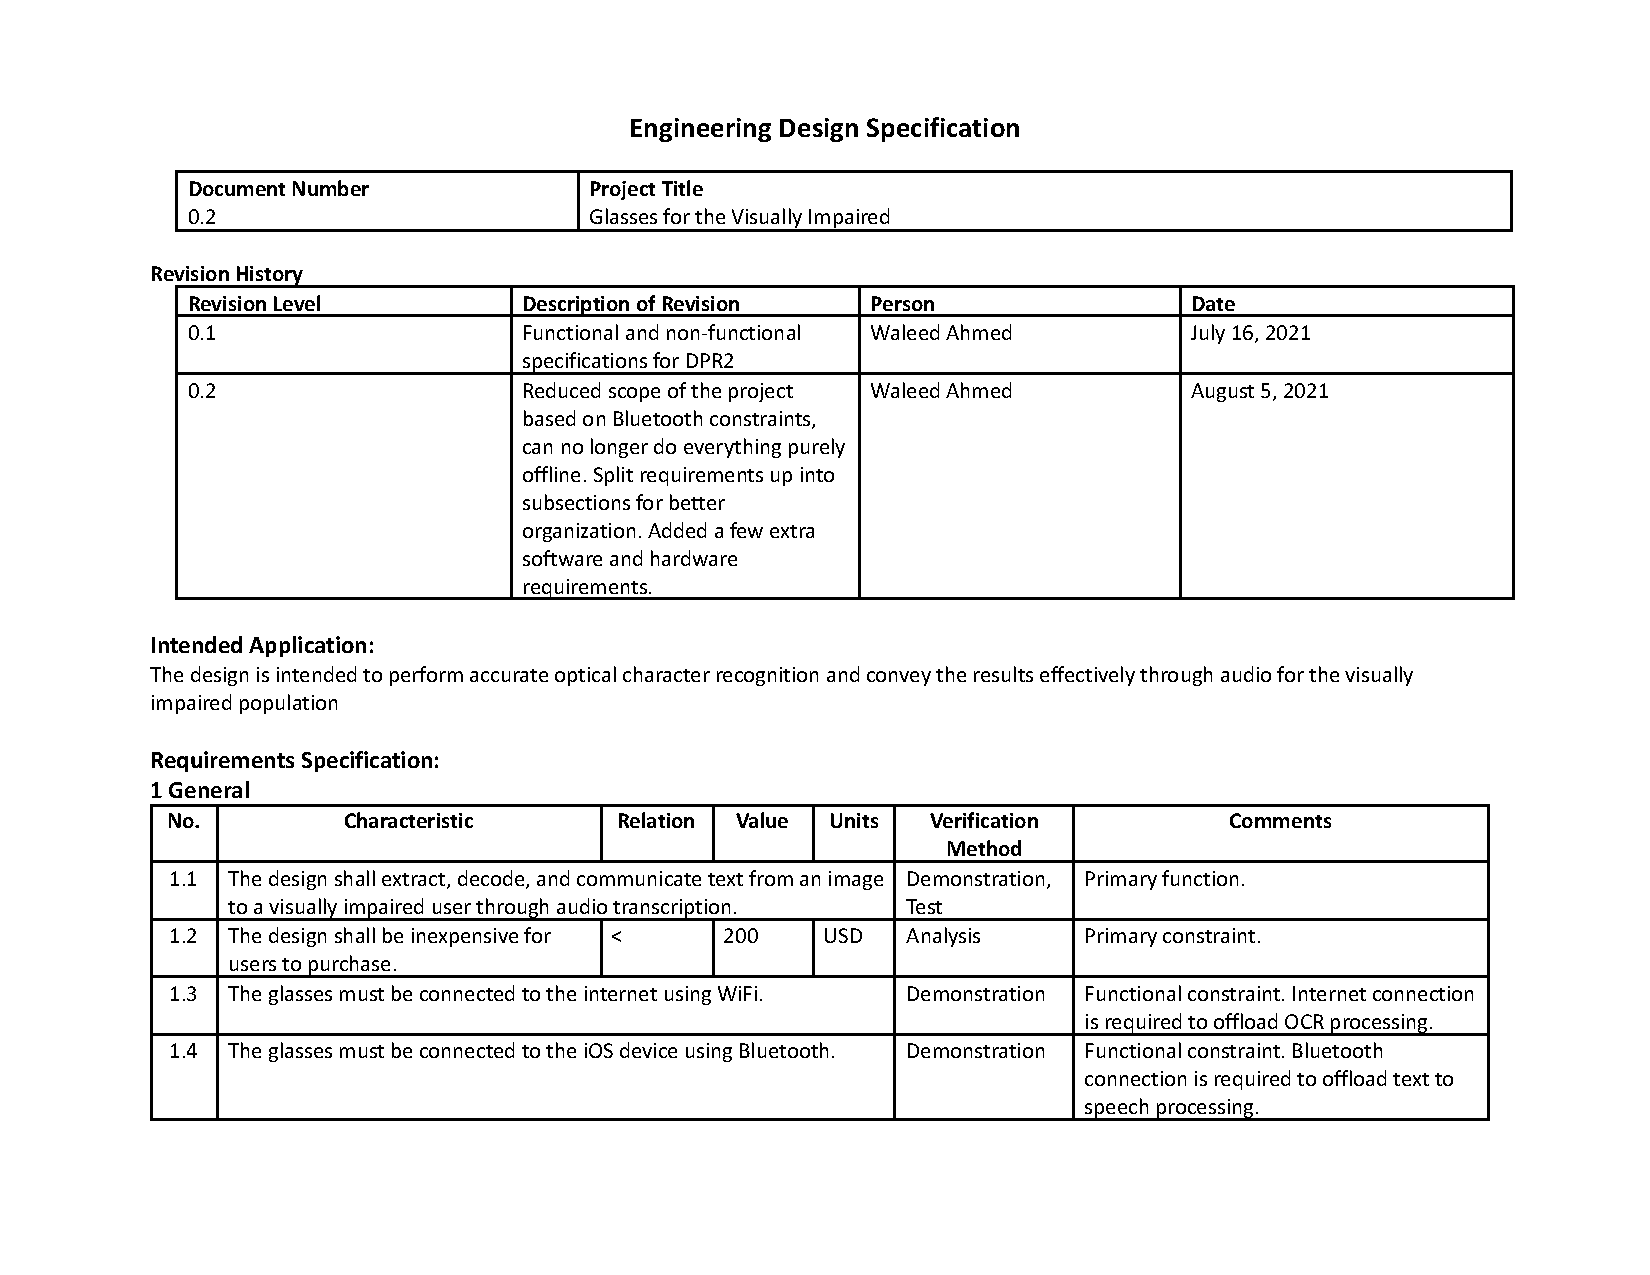
\includegraphics[page=1,width={0.86\linewidth}]{pdf/eds_0.2.pdf}
        \newpage
        \includegraphics[page=2,width={0.86\linewidth}]{pdf/eds_0.2.pdf}
        \newpage
        \includegraphics[page=3,width={0.86\linewidth}]{pdf/eds_0.2.pdf}
    \end{center}
\end{landscape}

\subsection{UI/UX Design}
\label{ui-ux-design}
The platform's UI and UX are designed around the fact that the users of our solution are universally visually impaired. This presented several unique design challenges and opportunities. For the hardware platform, we have decided to include two buttons built into the plastic housing that mounts to the side of a user's glasses. These can be used for capturing an image and performing OCR on it, switching between modes, powering the device on and off, etc. We plan to cement the functionality once we have a functioning hardware prototype. 

\

\noindent
When designing our software, we took advantage of the fact that all users would be incapable of seeing the phone's display, or at least incapable of seeing it clearly. Rather than building an app that is usable by sighted individuals and then adding tags/descriptions to make it usable with Apple's accessibility software, we designed the app around ease of use for the visually impaired. This meant adding extremely large buttons, so that rather than navigating to a smaller button which would be easy to press for a sighted person a user can simply tap either the top or bottom of the screen in order to activate a function.

\begin{figure}[H]
\centering
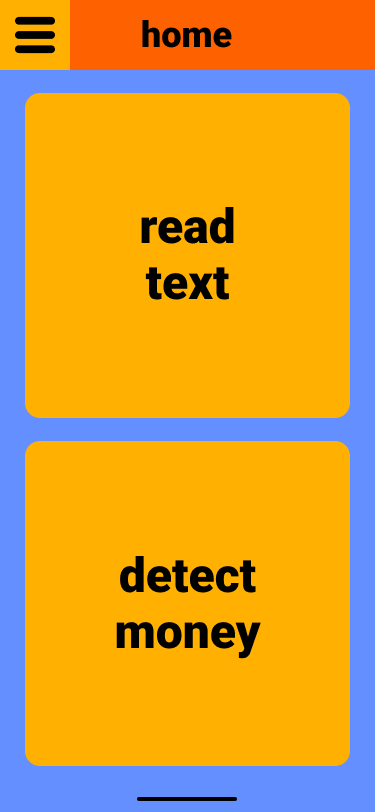
\includegraphics[scale=0.45]{img/main_screen_1.png}
\caption{Home Screen}
\label{fig:main_screen}
\end{figure}
\begin{figure}[H]
\centering
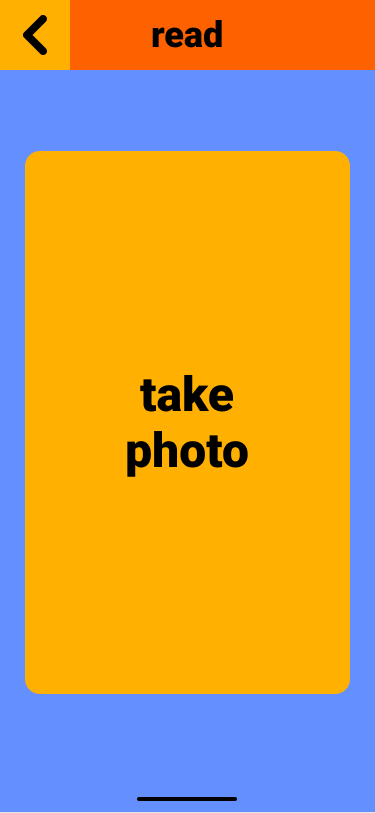
\includegraphics[scale=0.45]{img/read_screen_1.png}
\caption{Main Functionality Mockup}
\label{fig:read_screen}
\end{figure}

\noindent
We also plan to closely integrate our app with Apple's VoiceOver technology, which is their proprietary system for allowing blind or partially sighted people to interact with iOS devices. It reads items on the screen from left-to-right, top-to-bottom by default, although Apple exposes an API that allows developers to customize the order in which VoiceOver selects elements to interact with. The colour scheme [fig. \ref{fig:palette_standard}] was chosen to be functional for people with all 4 types of colourblindness [fig. \ref{fig:palette_deuteranopia}][fig. \ref{fig:palette_tritanopia}][fig. \ref{fig:palette_protanopia}][fig. \ref{fig:palette_greyscale}], while also having extremely high contrast so buttons can be distinguished from the background by partially sighted individuals.

\begin{figure}[H]
\centering
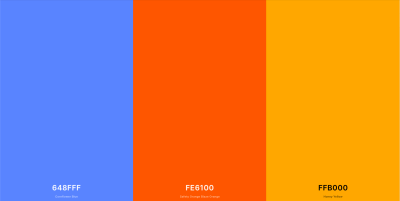
\includegraphics[scale=0.45]{img/Palette_Standard.png}
\caption{Colour Palette}
\label{fig:palette_standard}
\end{figure}
\begin{figure}[H]
\centering
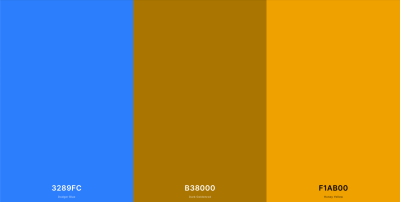
\includegraphics[scale=0.45]{img/Palette_Deuteranopia.png}
\caption{Palette (as viewed by someone with deuteranopia)}
\label{fig:palette_deuteranopia}
\end{figure}
\begin{figure}[H]
\centering
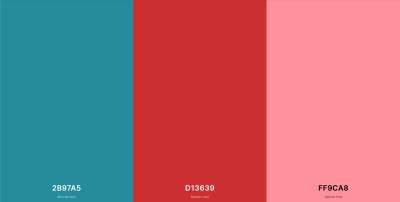
\includegraphics[scale=0.45]{img/Palette_Tritanopia.png}
\caption{Palette (as viewed by someone with tritanopia)}
\label{fig:palette_tritanopia}
\end{figure}
\begin{figure}[H]
\centering
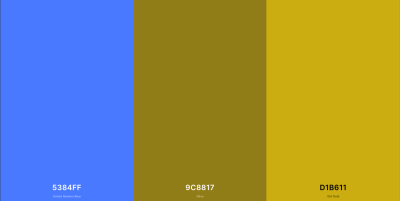
\includegraphics[scale=0.45]{img/Palette_Protanopia.png}
\caption{Palette (as viewed by someone with protanopia)}
\label{fig:palette_protanopia}
\end{figure}
\begin{figure}[H]
\centering
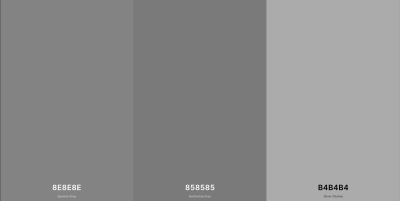
\includegraphics[scale=0.45]{img/Palette_Greyscale.png}
\caption{Palette (as viewed by someone with achromatopsia)}
\label{fig:palette_greyscale}
\end{figure}

\newpage
\section{Appendix B - Verification and Validation Data}

\subsection{OCR Testing}
Three OCR libraries were quickly tested out to get a quick idea of the performance and generalization capability of the library. At first, the Tesseract-OCR library \cite{tesseract-github} was tested but the predictions made by Tesseract were not accurate and so we decided to move on to a few other libraries. The two other libraries tested were PaddleOCR \cite{paddle-ocr} and EasyOCR \cite{easy-ocr}. Both libraries are built using Python. However, PaddleOCR is trained and deployed using a custom deep learning library called PaddlePaddle. Whereas EasyOCR is trained and deployed using a very popular library called PyTorch. Both libraries were evaluated on a machine text test image and a text-in-the-wild test image. The predictions from both libraries can be seen in Figures \ref{fig:eardrop_easyocr}, \ref{fig:kindle_easyocr}, \ref{fig:eardrop_paddleocr}, and \ref{fig:kindle_paddleocr}. Note that the visualizations were generated by the libraries themselves which is why they are different. However, by looking at the predictions, both libraries seem to perform well. However, since EasyOCR is built using PyTorch, it will be significantly easier to integrate into our app. Therefore, EasyOCR will be pursued in the near future.

\begin{figure}[H]
\centering
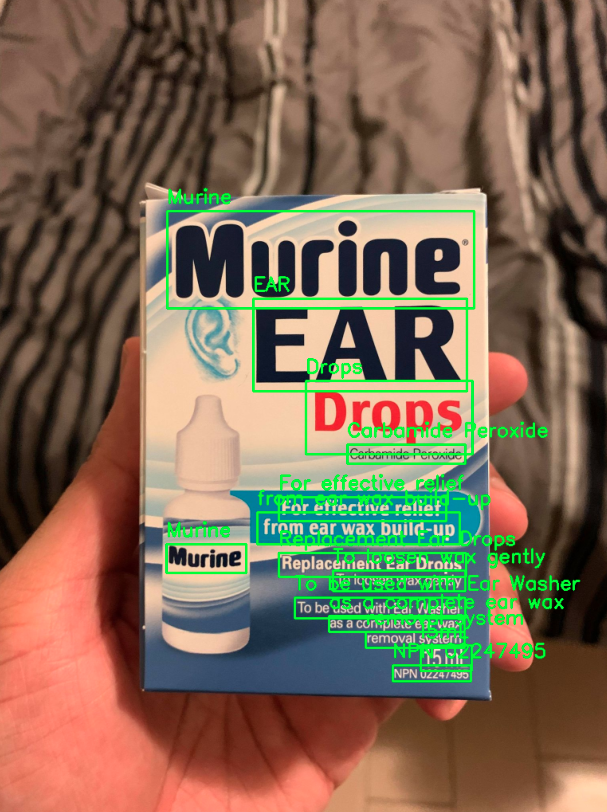
\includegraphics[scale=0.4]{img/ocr_testing/eardrop_easyocr.png}
\caption{EasyOCR prediction on the text-in-the-wild image.}
\label{fig:eardrop_easyocr}
\end{figure}

\begin{figure}[H]
\centering
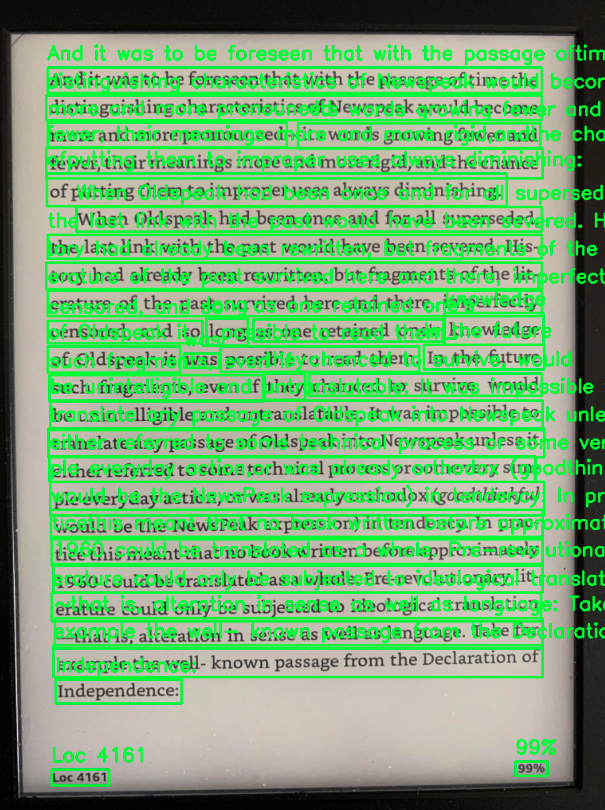
\includegraphics[scale=0.4]{img/ocr_testing/kindle_easyocr.png}
\caption{EasyOCR prediction on the machine text image.}
\label{fig:kindle_easyocr}
\end{figure}

\begin{figure}[H]
\centering
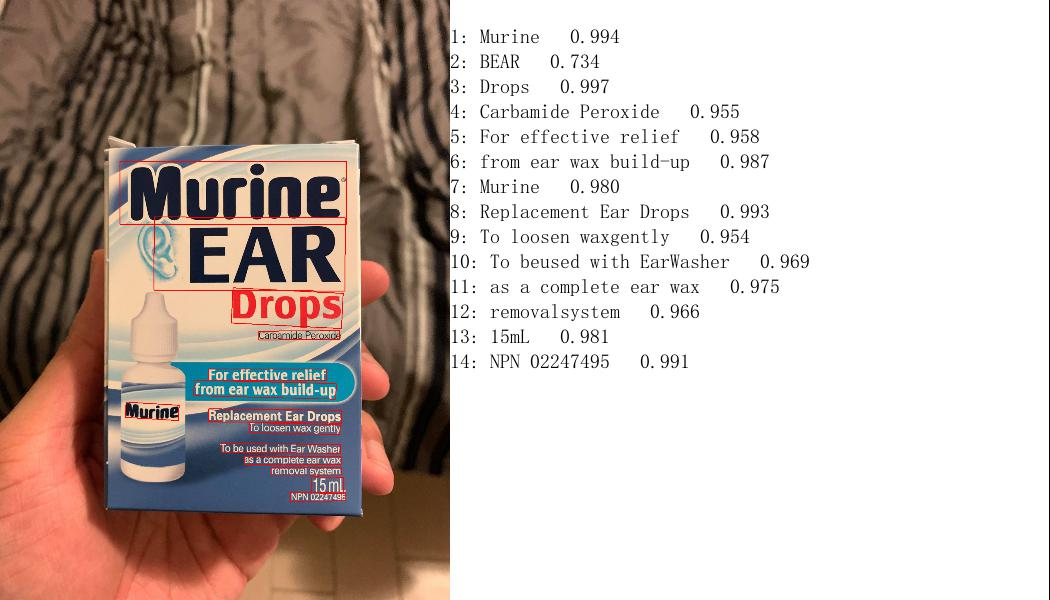
\includegraphics[scale=0.45]{img/ocr_testing/eardrop_paddleocr.jpg}
\caption{PaddleOCR prediction on the text-in-the-wild image.}
\label{fig:eardrop_paddleocr}
\end{figure}

\begin{figure}[H]
\centering
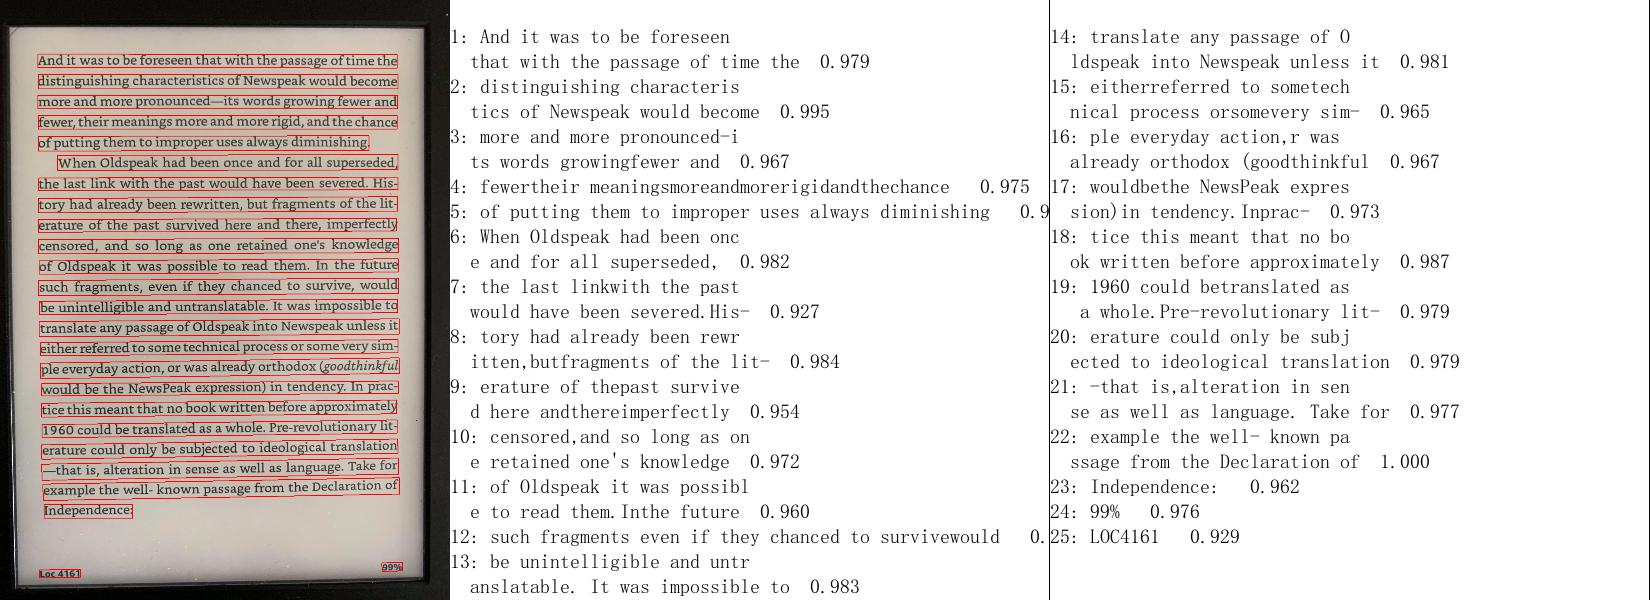
\includegraphics[scale=0.3]{img/ocr_testing/kindle_paddleocr.jpg}
\caption{PaddleOCR prediction on the machine text image.}
\label{fig:kindle_paddleocr}
\end{figure}

\noindent
Although evaluating a few images can give some idea of the performance of an OCR system, this is not a good way of evaluating a system. In the future, custom-built test sets will be created for both machine text and text-in-the-wild. These test sets will be used to evaluate various OCR methods and quantitatively decide on an OCR system. The metrics used to evaluate the OCR libraries are described in Section \ref{appendix-D}: Appendix D. The test sets will be built using images captured on the device to reduce the difference between our test sets and deployment environment. The test sets will also be built to purposefully reflect the use cases envisioned for the device.

\subsection{Installing Raspbian Lite on Raspberry Pi Zero W}
We used balencaEtcher software to flash an image of Raspbian Lite onto a 32GB micro-SD card. Raspbian Lite was used because we felt that there was no need for an operating system that included a graphical user interface. Additionally, given the relatively limited compute power available on the Raspberry Pi Zero W, a lighter version of Raspbian would be able to run more reliably.

\

\noindent
Once the OS image was flashed on the micro-SD card, we added two additional files:

\begin{itemize}
    \item ssh: This file would open a network port on the Raspberry Pi Zero W that accepts Secure Shell (ssh) connections, allowing us to use the Raspberry Pi Zero W remotely.
    \item wpa\_supplicant.conf: This file contains the information of the WiFi network available so that the Raspberry Pi Zero W can automatically search for and connect to the network.
\end{itemize}

\

\noindent
Once this initial setup was completed, the micro-SD card was inserted into the Raspberry Pi Zero W. Once it was connected to power, the Raspberry Pi Zero W would use the micro-SD card as a boot drive and initialize a file system, connect to the WiFi network, and open an ssh port for remote connections. Some additional configuration settings allow us to access the camera and install required packages and tools. At this point, the Raspberry Pi Zero W is ready for development.

\subsection{Bluetooth}
\label{bluetooth}
We had initially planned to use a Bluetooth Low Energy (BLE) connection to facilitate image transferring between the Raspberry Pi and the user's iOS device. We based this requirement around Apple's CoreBluetooth framework, and their restrictions on the amount of background processing iOS applications can perform. iOS has extremely aggressive memory and power management systems, which put apps into a suspended state when not in the foreground (i.e. when not open on the user's screen). Apple allows applications to request permission to perform background tasks, with certain limitations. One such permission is the ability to monitor communications from a paired BLE peripheral and act upon incoming data \cite{apple-bluetooth}. Once an incoming BLE packet destined for an application is detected, iOS provides a 15-30 second window for said application to complete any tasks it needs to do to react to this data before putting them back into a suspended state automatically.

\

\noindent
We had planned to compress an image into JPEG format on the Raspberry Pi, then send a BLE notification to the iOS device that a new image was available for processing. The iOS device would then wake up the background application and pass along the BLE packet. The iPhone could then connect to the Raspberry Pi and retrieve the image. However, we discovered that BLE's extremely lightweight nature makes it impractical for transmitting large files (such as an image). The Raspberry Pi uses a Bluetooth 4.1 chip \cite{raspi-hardware}, which imposes a limit on the size of the data field in a transmitted BLE packet. The iPhone has a Bluetooth 4.2 chip \cite{iphone-hardware} which is capable of communicating with the Raspberry Pi's older chip, but is rate limited by the Pi's hardware. The maximum size of a data field in a packet sent between the two devices is therefore 27 bytes, although 4 of these bytes are used to store an offset (so that files larger than 27 bytes can be sent using consecutive packets. Additionally, iOS allows a maximum of 4 packets to be exchanged before a new BLE connection needs to be made. The BLE protocol also mandates a connection interval, which varies by device but is set to 15ms on all devices running iOS 11 or later \cite{apple-bluetooth}. This means that it would take almost a minute to transmit the smallest photo we could reasonably perform OCR on. This falls outside the window that iOS provides for a device to perform processing, before the application even receives the image.

\

\noindent
We have come up with several solutions to this problem, although they all revolve around having a WiFi connection. These include having the Raspberry Pi communicate directly with a server, uploading an image, and processing it in the cloud. The main drawback of this solution is that the system will not work offline, which was a functional requirement for our project. We have decided to redefine this requirement as a feature that would exist in the final product, but one that we are unable to implement in the prototype. The reasoning behind this decision is explained in section \ref{apple-mfi}.

\subsection{Apple MFi}
\label{apple-mfi}
Bluetooth Classic is a different version of Bluetooth which supports much higher throughput; BT Classic connections are two-way, continuous data streams up to 2.1Mbps \cite{bluetooth-classic}. iOS supports this version of Bluetooth, although it is restricted to embedded chips with Apple's MFi (Made For iPod) certification \cite{apple-mfi}. Using Bluetooth Classic would provide the data transfer speeds needed to send an image quickly enough to provide a good user experience, although the ability to perform background processing is restricted to BLE devices. Nevertheless, this would enable us to perform OCR on a piece of text and read it back while the user is offline. In our final product, we would apply for an Apple MFi certification in order to unlock the full potential of Bluetooth on iPhone.

\newpage
\subsection{iOS Test App}
In order to try various OCR libraries and speech synthesis in iOS, a small bare-bones test application was made. The app allows you to take a picture with the phone's camera or use the photo library. The image is lightly pre-processed (rescaled and converted to grayscale to improve OCR performance \cite{tesseract-improve-quality}), then run through Tesseract OCR, a well known open source OCR library currently maintained by Google \cite{tesseract-github}. Tesseract outputs a string containing the detected text, and Apple's native speech synthesis library \cite{apple-speech-synthesis} is then used to convert the text to audio and then play the audio to read out the text.

\

\noindent
Below are some screenshots from the app to showcase it's functionality. The blue camera button in the top right is what allows you to select a photo from library or take one using the camera.
\begin{figure}[H]
    \centering
    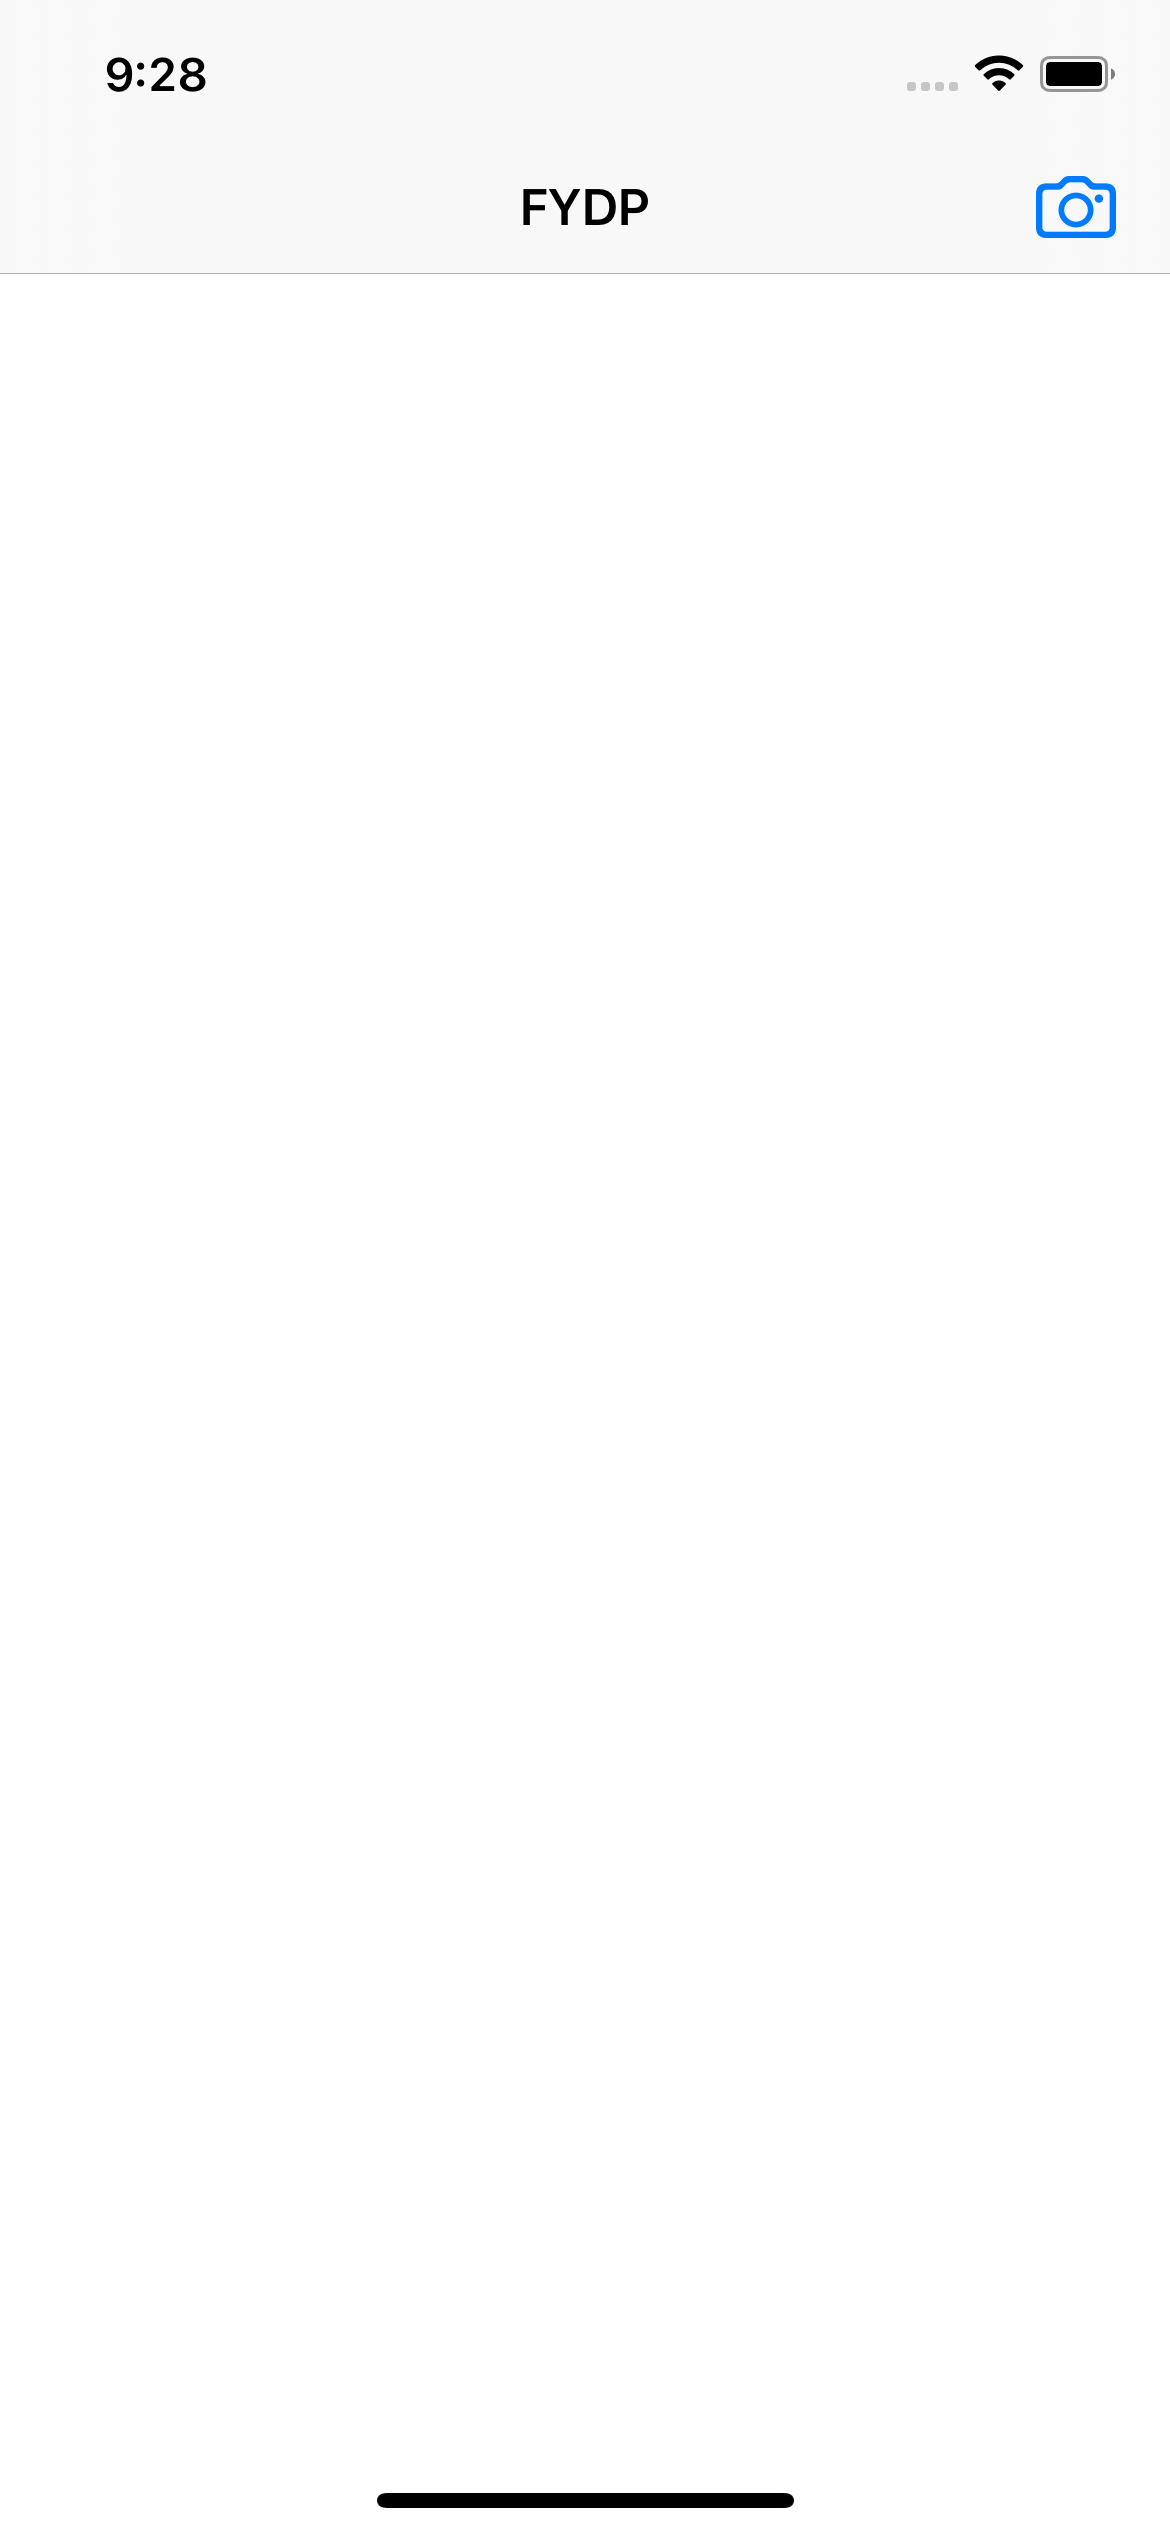
\includegraphics[width={0.3\linewidth}]{img/ios_test_app/testapp_home.png}
    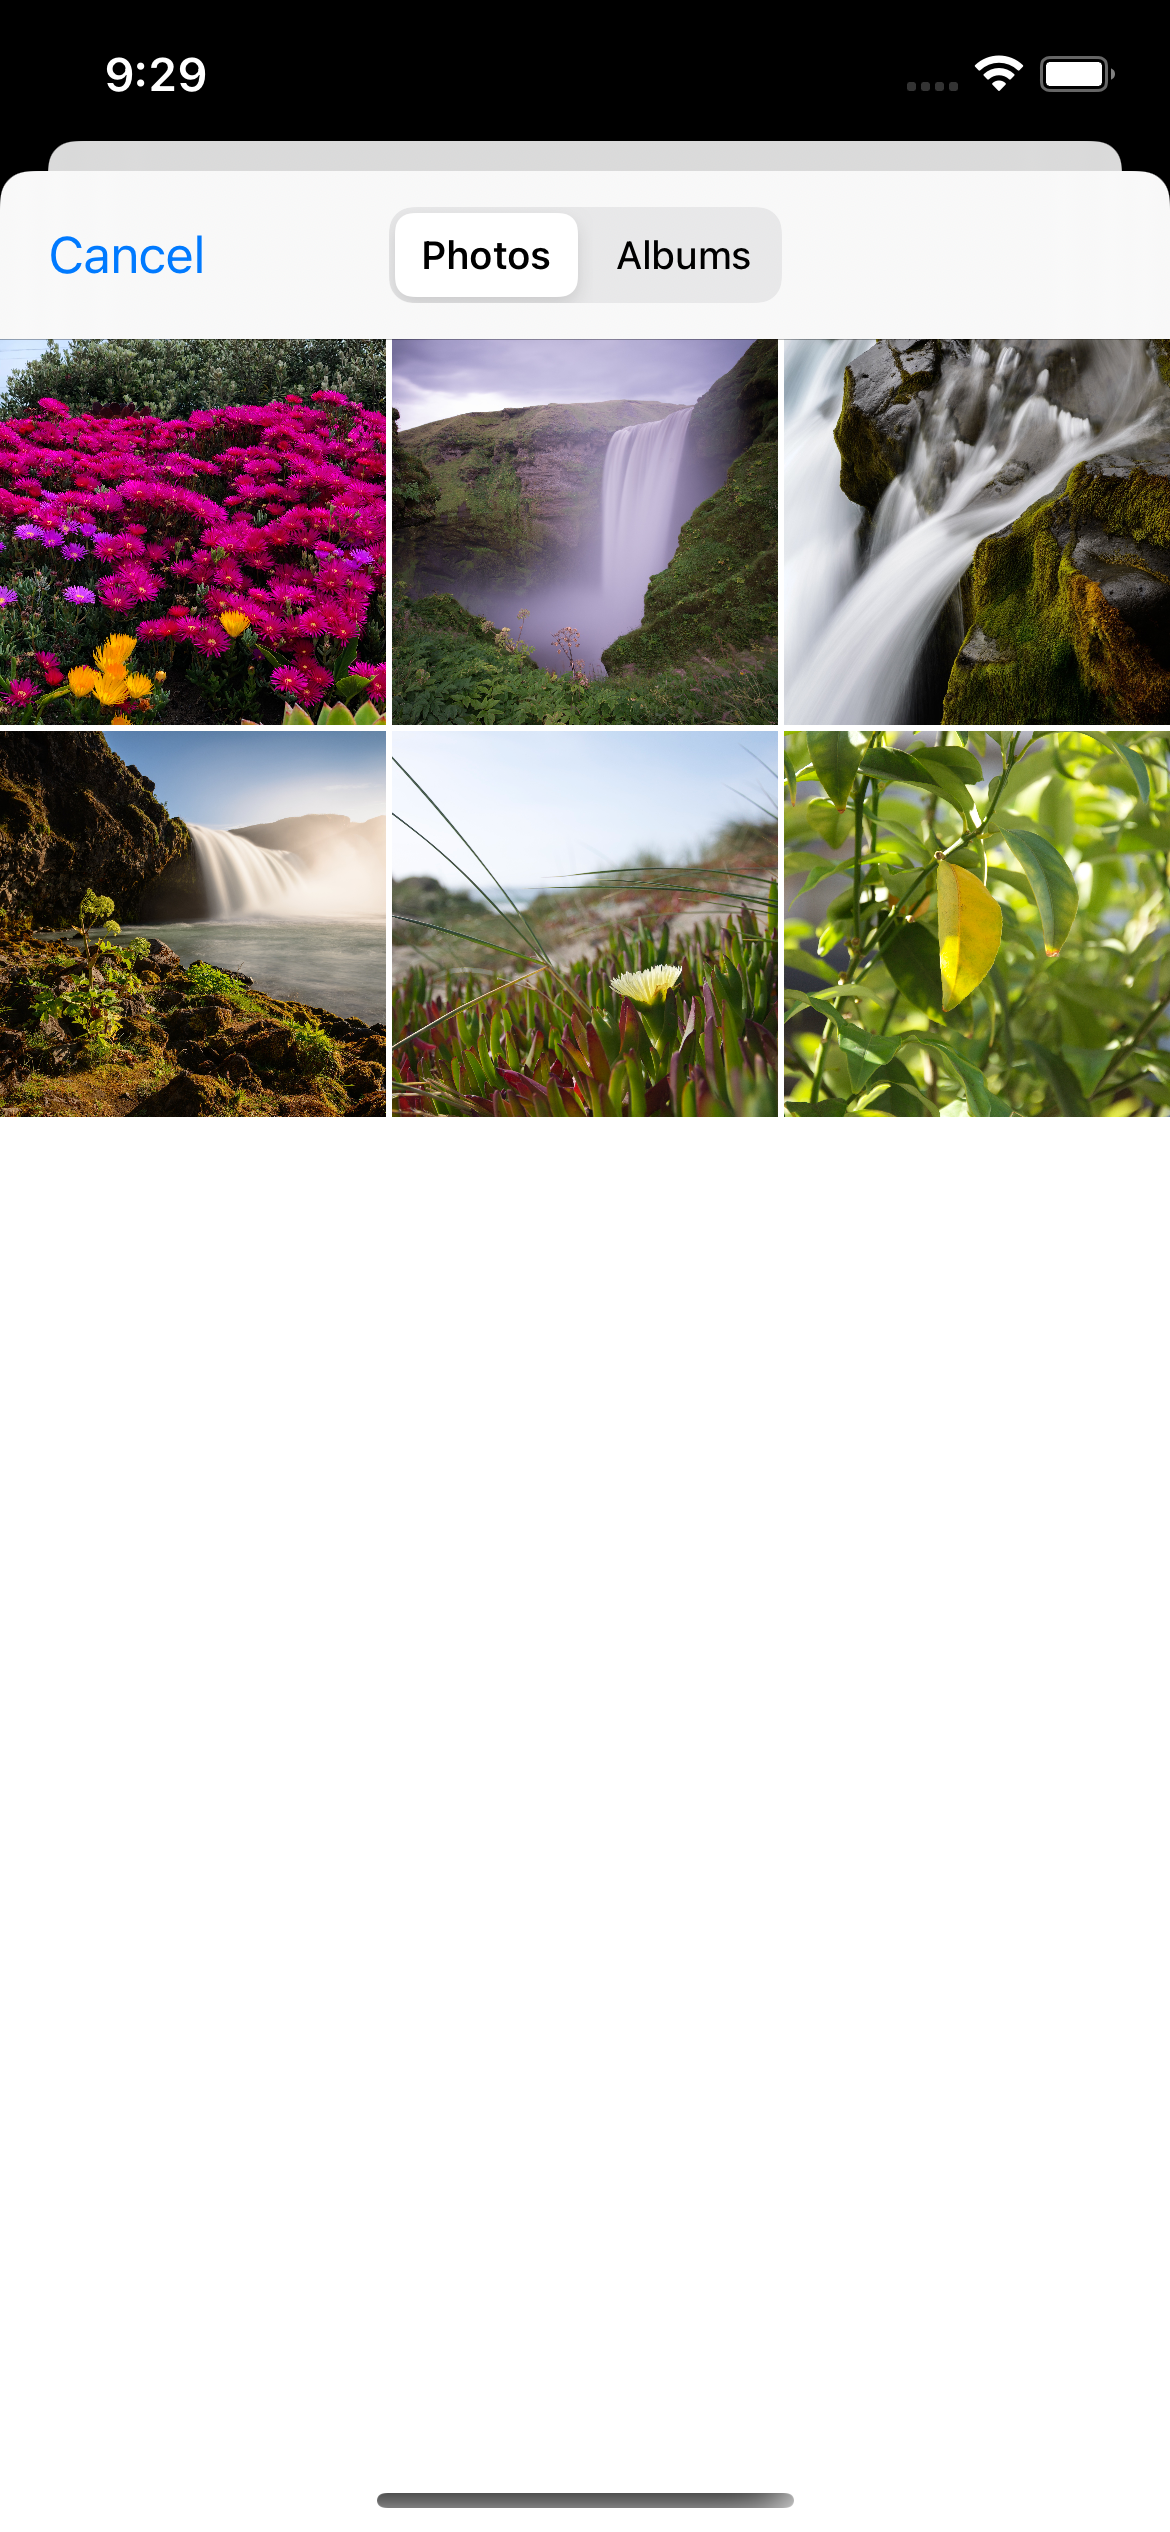
\includegraphics[width={0.3\linewidth}]{img/ios_test_app/testapp_library.png}
    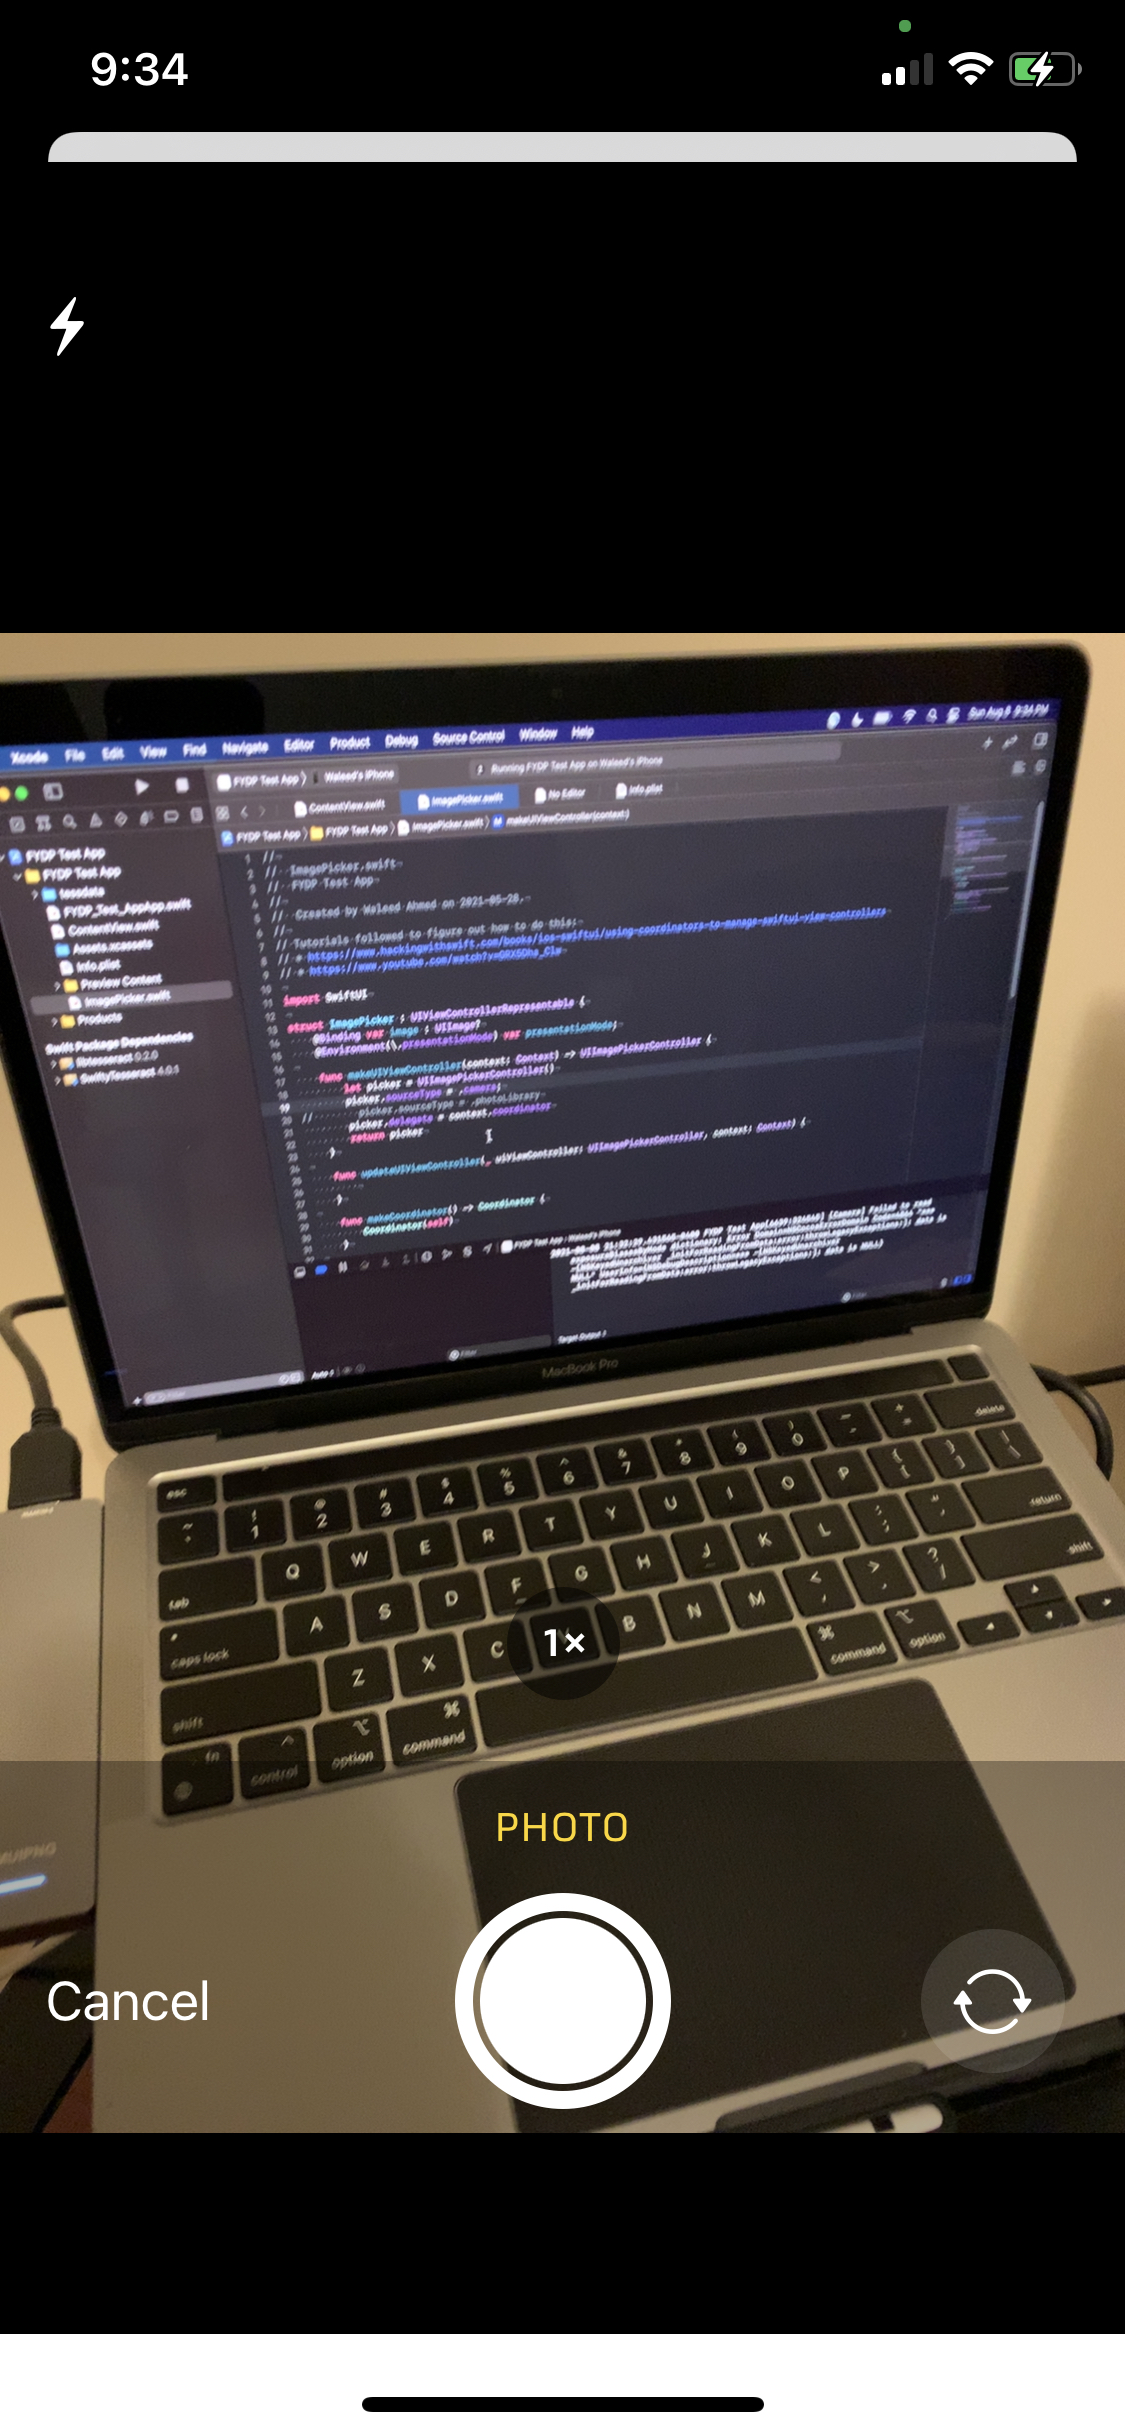
\includegraphics[width={0.3\linewidth}]{img/ios_test_app/testapp_photo.jpeg}
    \caption{Left to right: home screen, pick photo from library, take photo with camera}
\end{figure}

\newpage
\noindent
Below are two examples of OCR being done on machine text and text in the wild within the app:

\begin{figure}[H]
    \centering
    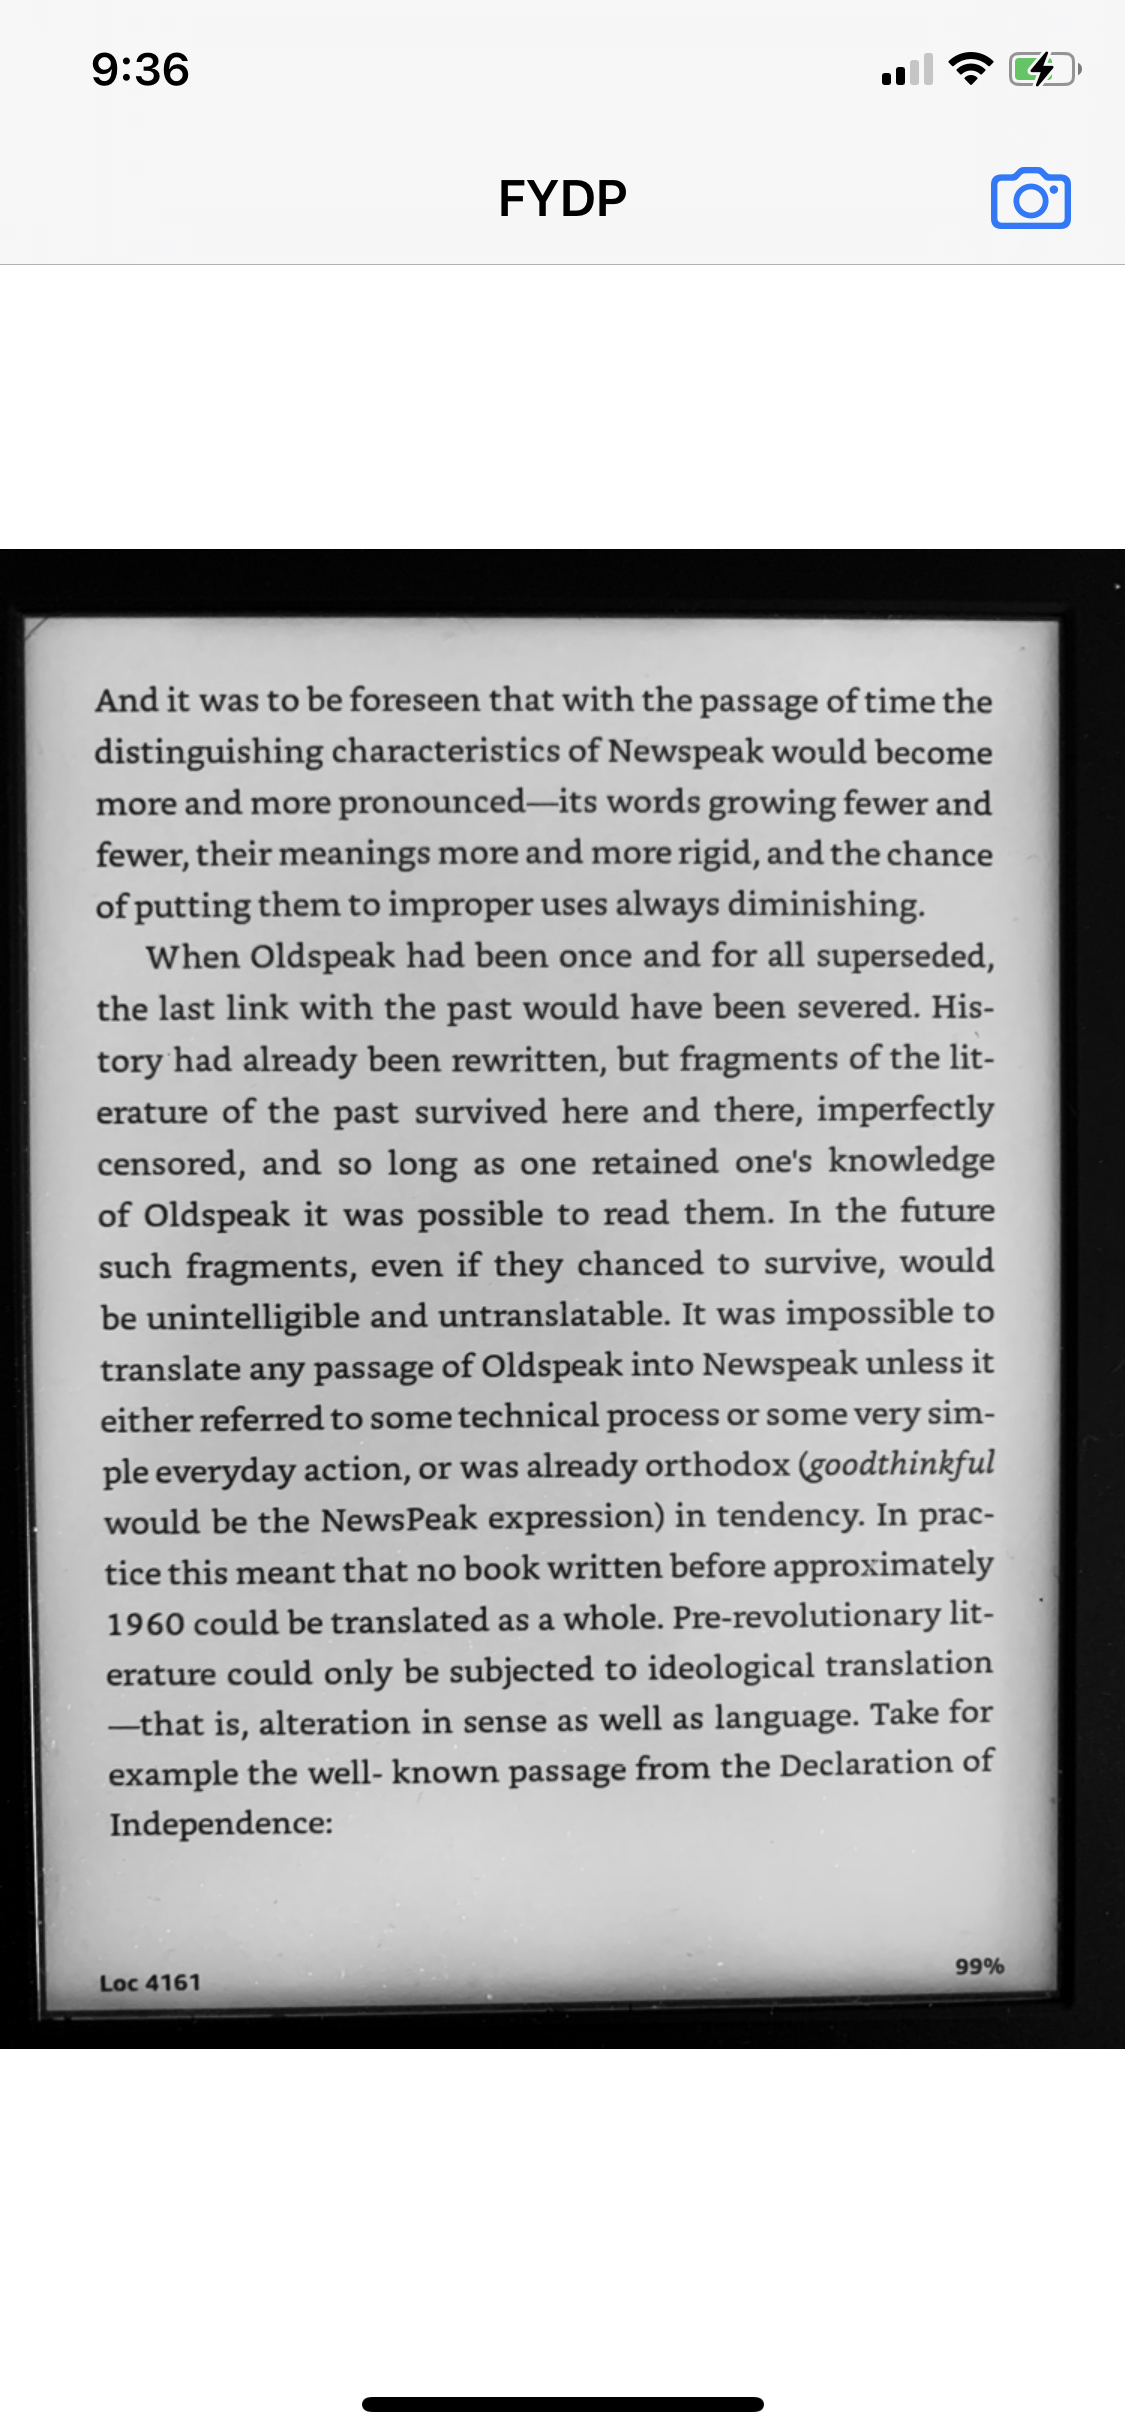
\includegraphics[width={0.25\linewidth}]{img/ios_test_app/testapp_kindle.jpeg}
    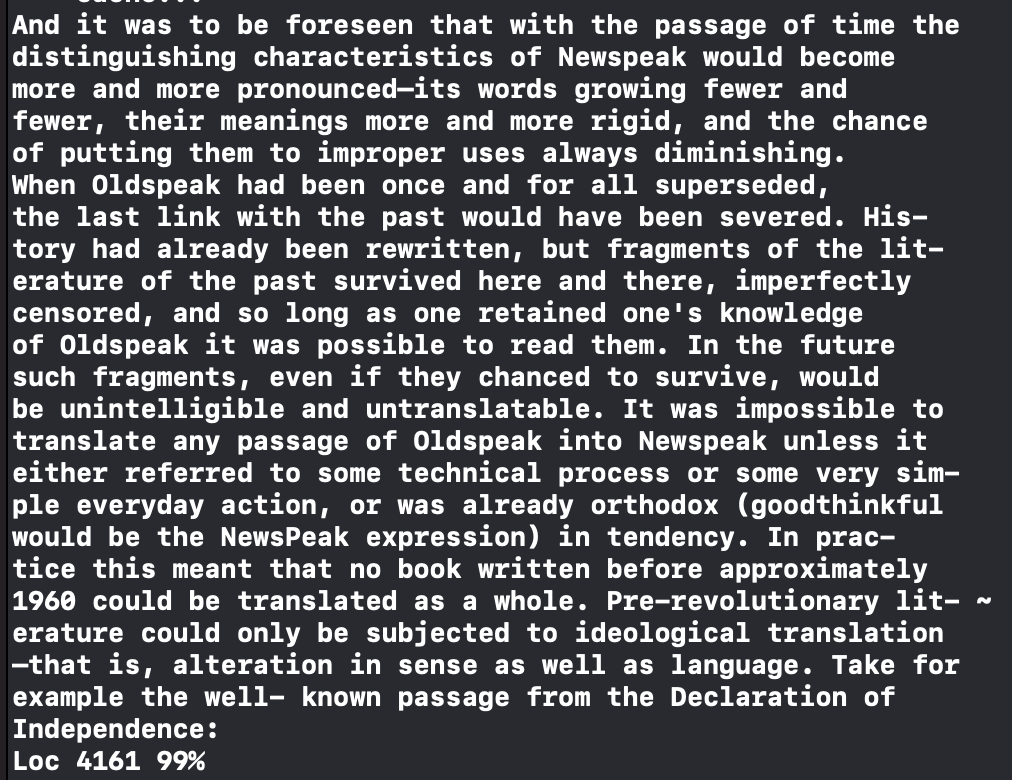
\includegraphics[width={0.5\linewidth}]{img/ios_test_app/testapp_kindle_output.png}
    \caption{Machine text example. Left: app screenshot, Right: OCR output printed in Xcode console}
    \label{machine-text-ios-example}
\end{figure}

\begin{figure}[H]
    \centering
    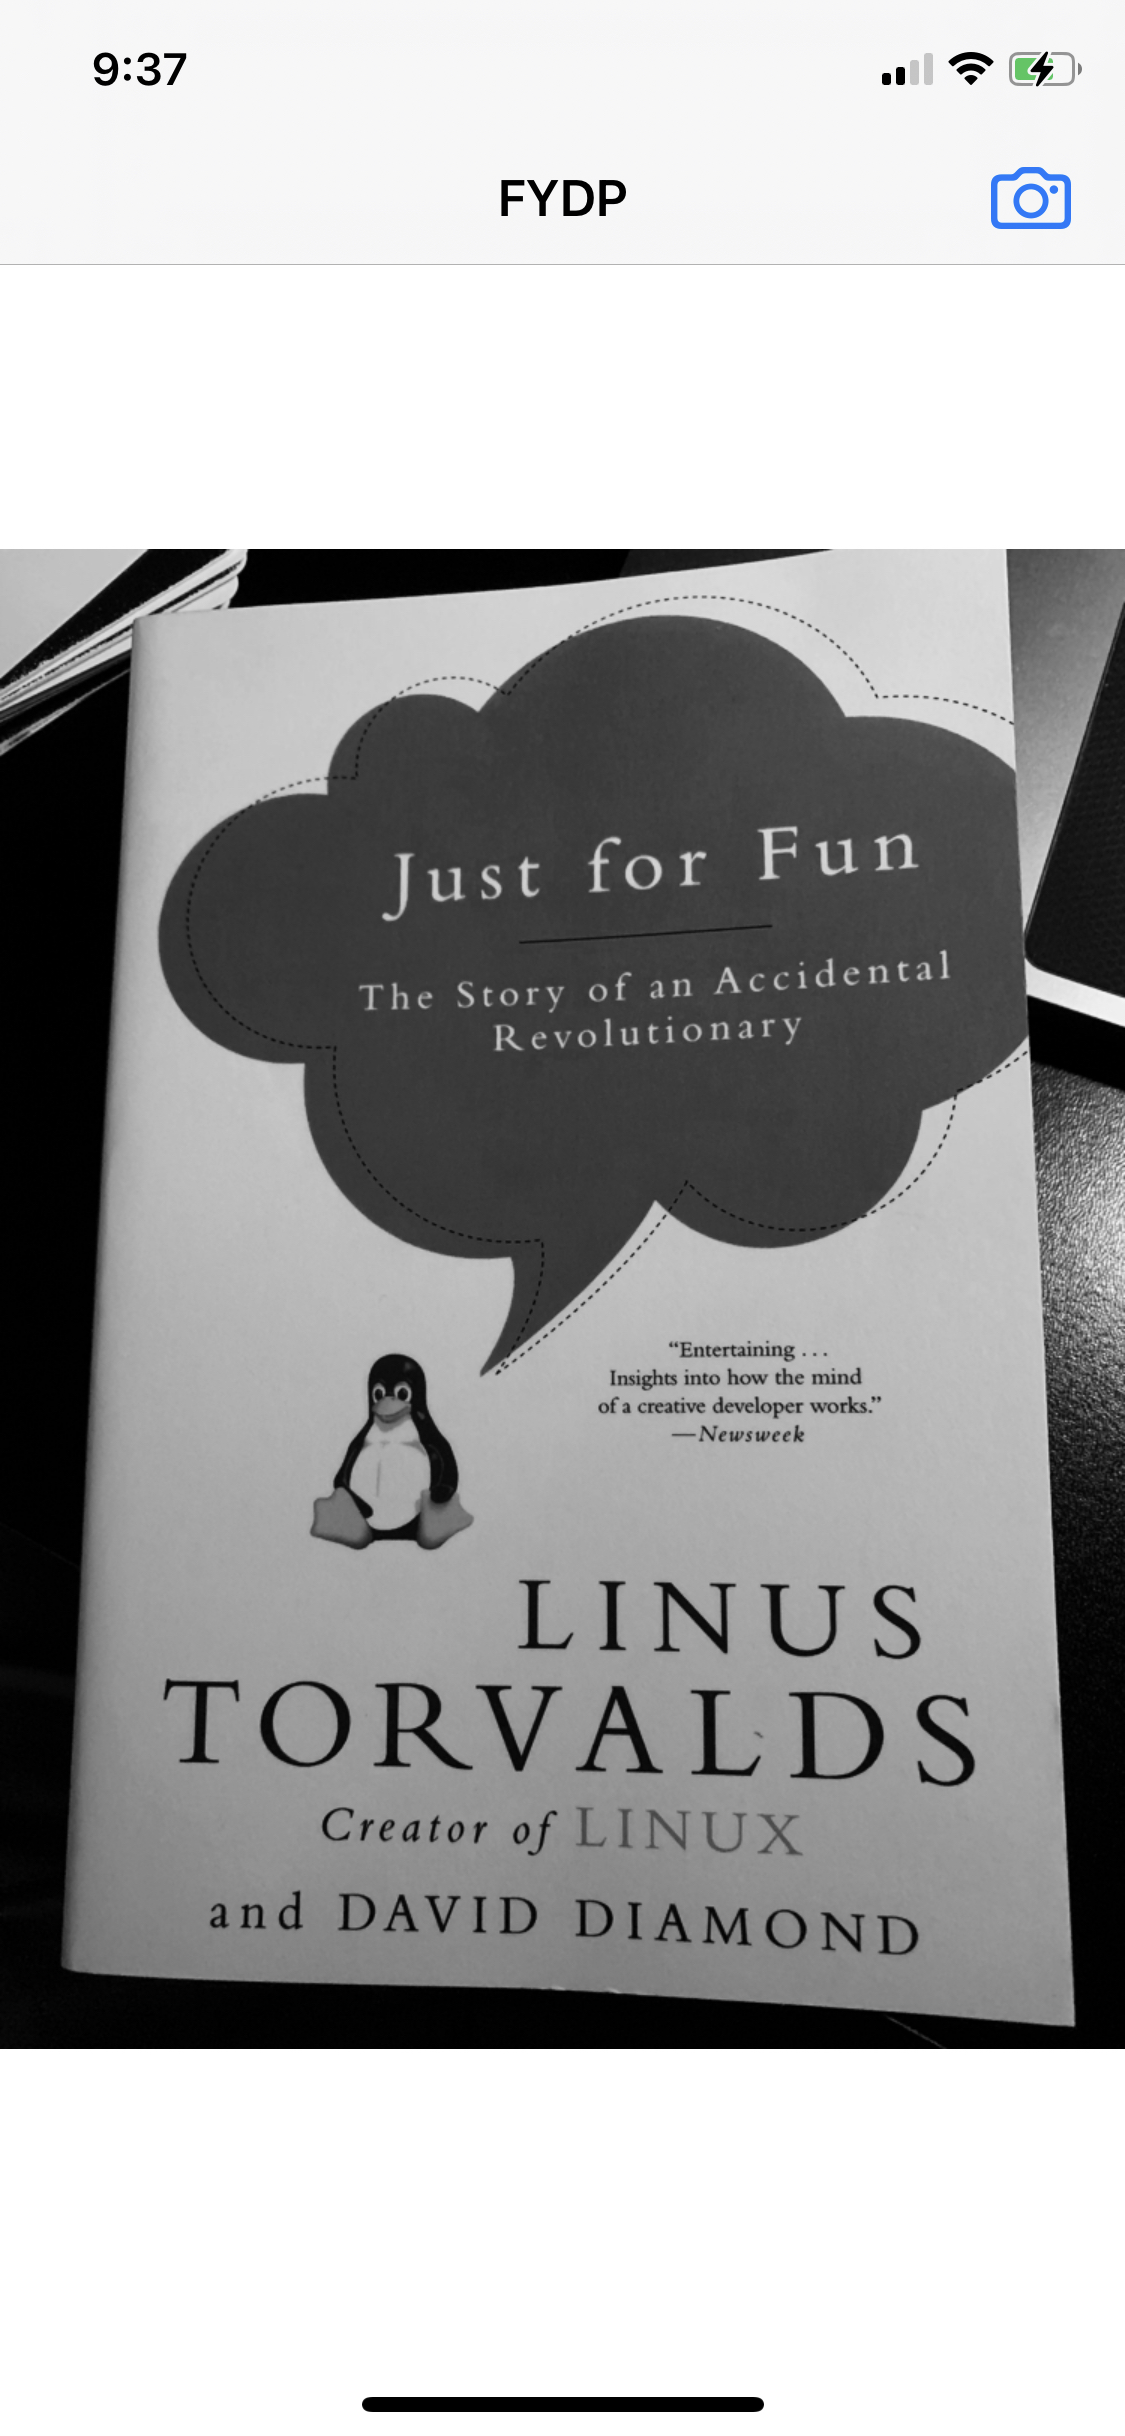
\includegraphics[width={0.25\linewidth}]{img/ios_test_app/testapp_bookcover.jpeg}
    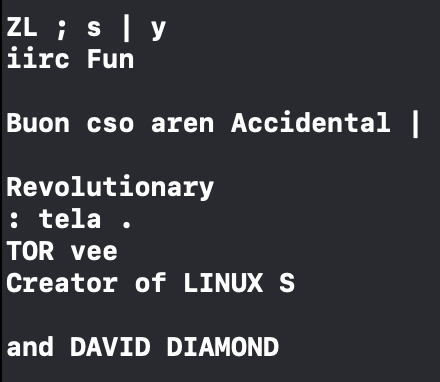
\includegraphics[width={0.5\linewidth}]{img/ios_test_app/testapp_bookcover_output.png}
    \caption{Text in the wild example. Left: app screenshot, Right: OCR output printed in Xcode console}
    \label{text-in-the-wild-ios-example}
\end{figure}

\noindent
As shown by figures \ref{machine-text-ios-example} and \ref{text-in-the-wild-ios-example}, Tesseract OCR performs well on machine text, but not on text in the wild. Handwritten text was also tested, but it returned garbage. Tesseract OCR is one of the older OCR engines and was mostly trained on well-formed machine text, so it doesn't generalize well to text in the wild. We are very likely not going with this as our OCR engine, it was simply easy to set up and test in iOS, so we tried it out first.

\ 

\noindent
The entire pipeline of taking the photo, pre-processing, and performing speech synthesis runs relatively fast on most images. On Waleed's iPhone XS, this pipeline runs in about 1 second depending on the image. This showed us that this pipeline is feasible to run and can return results quickly to the user. Note however that this is not our final pipeline, as we are no longer planning on running the OCR engine on the phone, due to Bluetooth Low Energy limitations of sending the image from the glasses to the phone. However, if we decide to support the usage of the phone's camera in the final app, the infrastructure from this test app can be leveraged.

\

\noindent
Click \href{https://youtu.be/mMBuUgM9Zts}{here} to see a demo of the app. Note that other voice options are available for the speech synthesis, the one used in this demo is the British English voice. We will likely allow the user to customize the voice and test out various ones to see which one is the most natural-sounding to use as the default.

\subsection{Electrical Validation}
\label{elec-verification}
As part of keeping the device safe for use, part of our validation effort will be to monitor the current draw of the device as operation approaches our final desire workload. We will be using a USB tester shown in figure \ref{fig:usb-tester}.

\begin{figure}[H]
\centering
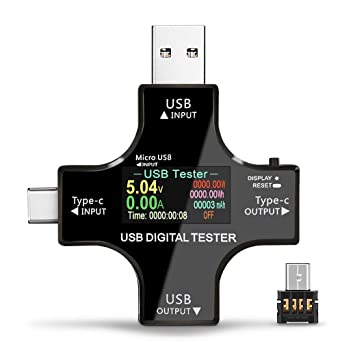
\includegraphics[scale=0.6]{img/USB tester.jpg}
\caption{USB Tester Device}
\label{fig:usb-tester}
\end{figure}

\noindent
This device can measure the real-time operating voltage, current draw, and is able to calculate power consumption in 3 different units: Watts, Watt-hours, and milliamp-hours. The latter is extremely useful to us as we will be using a battery to power the device, and our battery life can be effectively measured by extrapolating from power draw measurements.



\newpage
\section{Appendix C - Design Project Management Data}
\label{appendix-c}

\subsection{Summary of Software and Tools Used}
We are using many tools for configuration management and record keeping. They are all listed below:

\begin{itemize}
    \item Discord: Internal meetings and communication.
    \item Notion: Meeting and research notes. See Section \ref{meeting-logs} for more on our Notion setup.
    \item ClickUp: Tasks and timelines. See Section \ref{schedule} for more info.
    \item Overleaf: LaTeX editor to create and store reports.
    \item Google Drive: Store files, presentation slides, and revision controlled documents such as the engineering design specification and risk register.
    \item Github: Source code and software documentation.
    \item Microsoft Teams: Meetings with faculty advisor.
\end{itemize}

\subsection{Schedule}
\label{schedule}

\subsubsection{Original Timeline}
The original timeline (developed and presented at design project review 1) is included for completeness and to illustrate timeline changes.
\begin{center}
    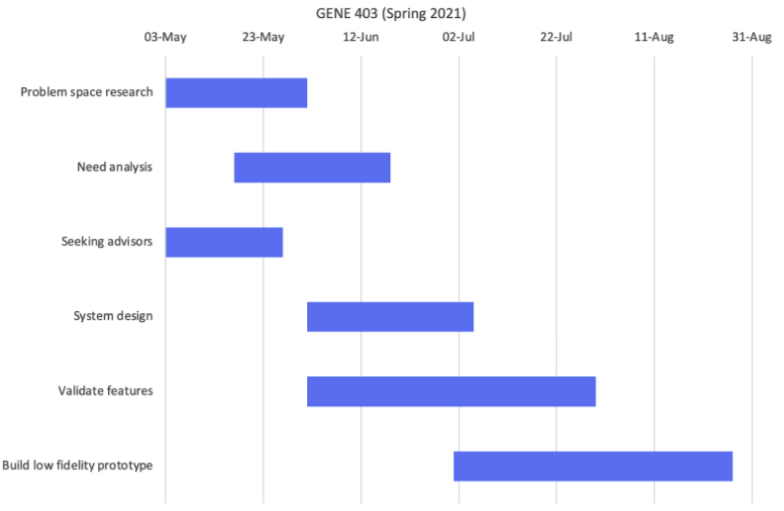
\includegraphics[width={0.5\linewidth}]{img/s21-timeline.png}
    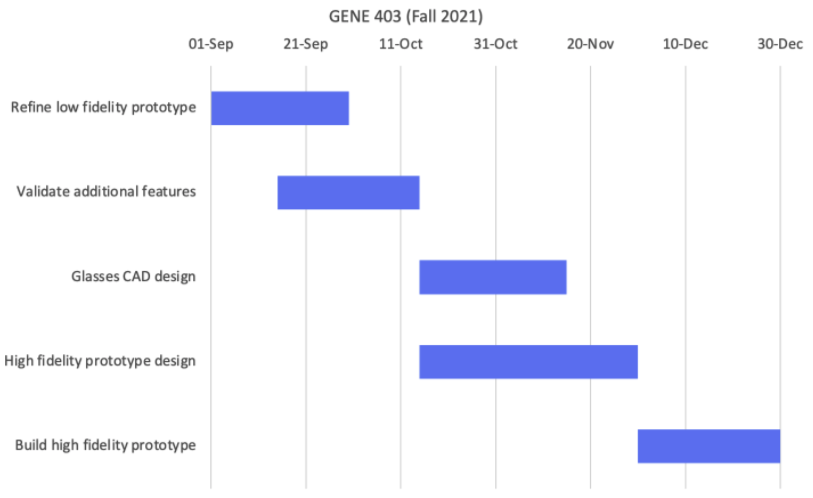
\includegraphics[width={0.5\linewidth}]{img/f21-timeline.png}
    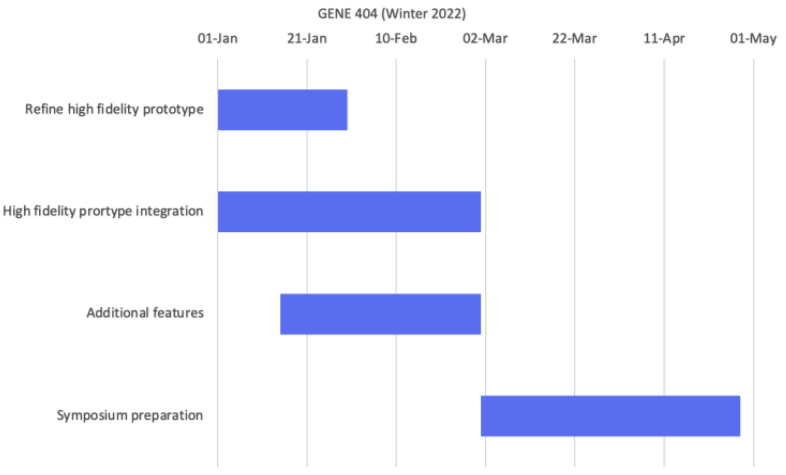
\includegraphics[width={0.6\linewidth}]{img/w22-timeline.png}
\end{center}

\subsubsection{Current Timeline}
\label{current-timeline}

We started using ClickUp \cite{clickup} near the end of the term as our primary product management software to keep track of timelines and tasks. Below are the gantt charts showcasing the current high level timeline as well as subsystem level tasks for Software and Hardware. Note that these will be continually evolving as our project progresses, this is just a current snapshot of where we are at.
\begin{center}
    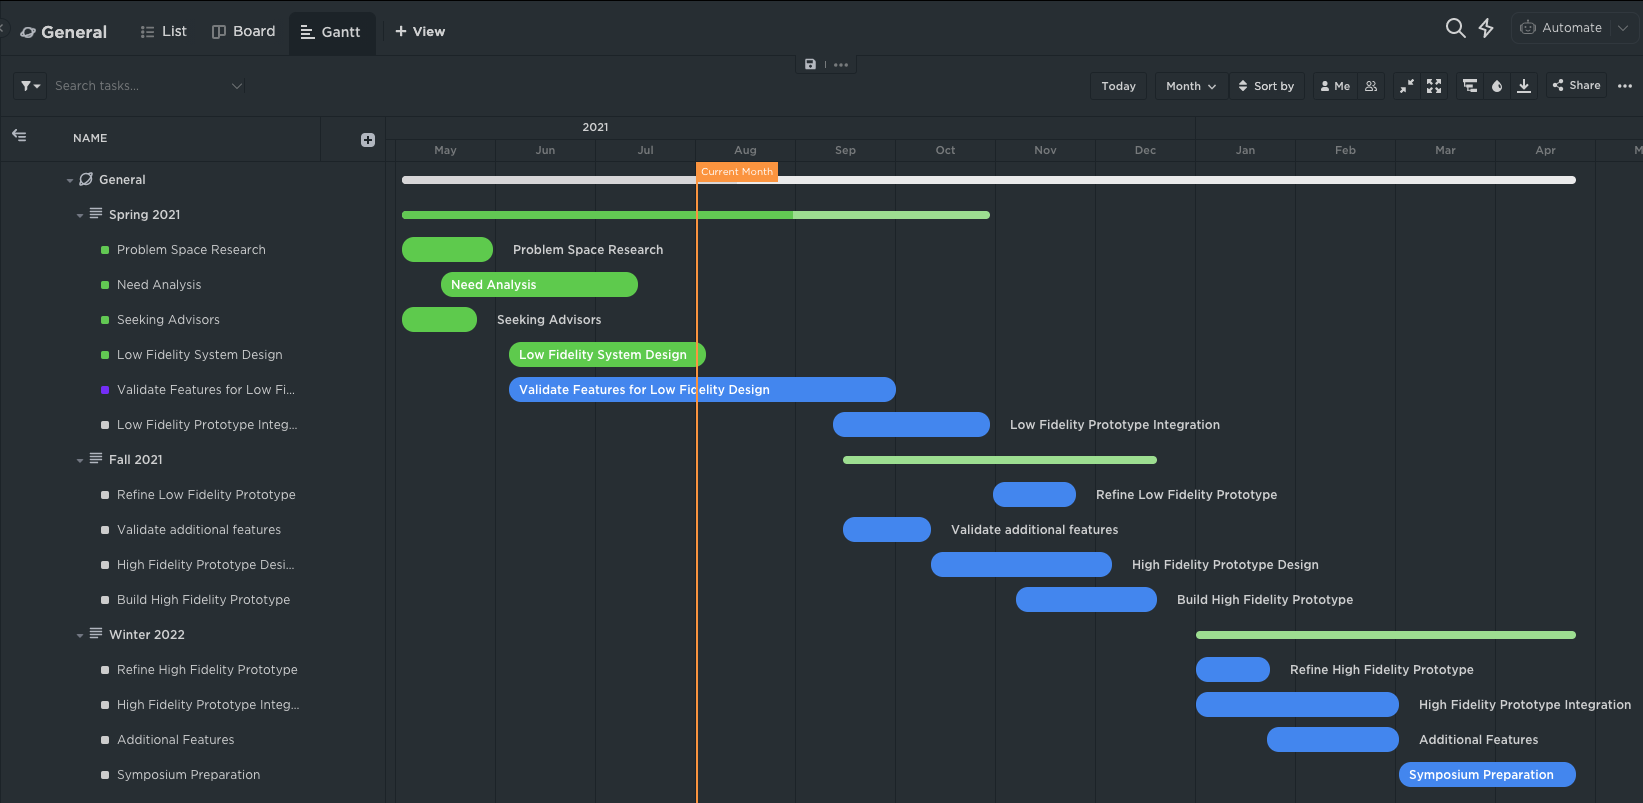
\includegraphics[width={1.0\linewidth}]{img/general-gantt.png}
    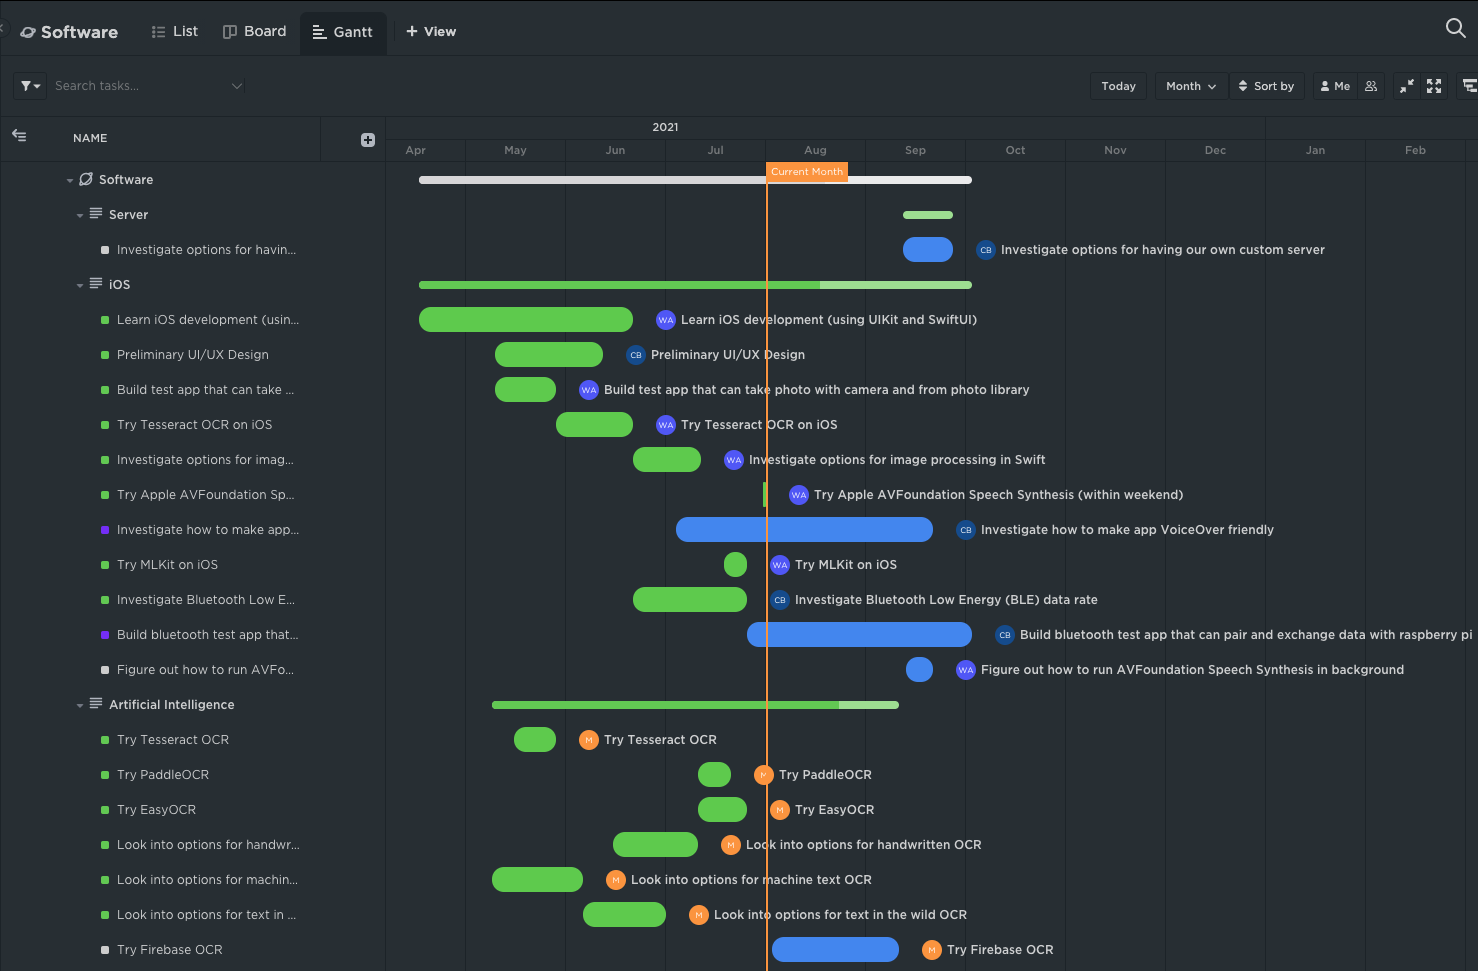
\includegraphics[width={1.0\linewidth}]{img/software-gantt.png}
    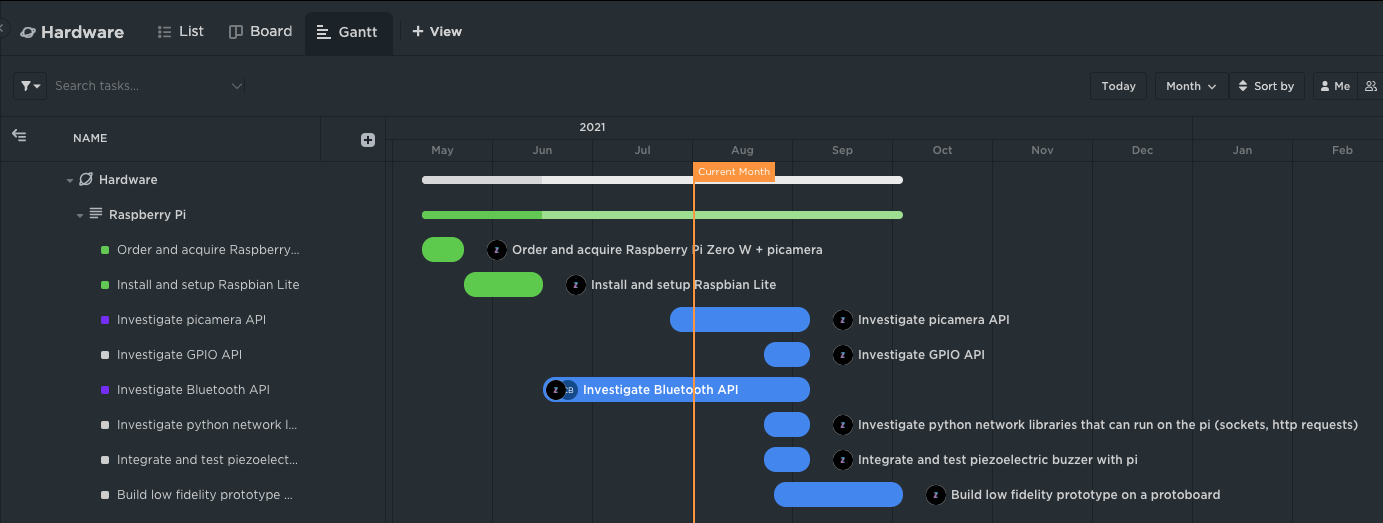
\includegraphics[width={1.0\linewidth}]{img/hardware-gantt.png}
\end{center}


\newpage
\subsection{Budget}
Table \ref{Tab:budget} shows a breakdown of all materials and resources purchased and/or used during the Spring 2021 Academic Term for the purpose of the project.

\begin{table}[ht]
    \centering
    \begin{tabular}{|l|c|r|}
        \hline
        
        \textbf{Item / Resource} & \textbf{Supplier} & \textbf{Cost (CAD)}
        \\ \hline
        Raspberry Pi Zero W Camera Pack & Adafruit      & 44.95
        \\ \hline
        SanDisk Ultra 32GB micro SDHC   & Amazon        & 12.79
        \\ \hline
        UGREEN Mini HDMI Adapter        & Amazon        & 10.99
        \\ \hline
        Electop USB Power Meter Tester  & Amazon        & 29.36
        \\ \hline
        Github Organization Free        & Github        & 0
        \\ \hline
        ClickUp Workspace               & ClickUP       & 0
        \\ \hline
        Overleaf Online LaTeX Editor    & Overleaf      & 0
        \\ \hline
        Labour Costs                    & N/A           & 15,120
        \\ \hline
        \textbf{Total}                  & \multicolumn{2}{r|}{\textbf{15218.09}}
        \\ \hline
    \end{tabular}
    \label{Tab:budget}
\end{table}
\noindent
As a note, Labour costs were estimated using a rate (per student) of \$35/hour, 9 hour/week workload, and a 12-week term.

\

\noindent
For the upcoming Fall 2021 and Winter 2022 terms, our budget estimate is \$15,220/term. This is estimated using the same Labour Costs, and an additional \$100/term for any additional hardware components that may need to be purchased.

\subsection{Organizational Chart}
\begin{table}[ht]
    \centering
    % \begin{tabular}{|c|c|c|c|}
    \begin{tabular}{|p{2.8cm}|p{5.5cm}|p{6.5cm}|}
        \hline
        Name & Position & Responsibilities \\ \hline
        Waleed Ahmed & Project Manager & Driving discussions, scheduling, brainstorming, meeting logs, general support on prototyping and integration
        \\ \hline
        
        Martin Ethier & Artificial Intelligence Lead & 
        Research, testing, and integration of artificial intelligence software
        \\ \hline
        
        Zain Denno & Hardware and Embedded Lead & 
        Research, testing, and integration of the hardware platform \\ \hline
        
        Connor Barker & iOS Lead & 
        Research, testing, and integration of the mobile iOS application \\ \hline
        
        John Zelek & Faculty Advisor (SYDE) & Problem space and technical consultation \\ \hline
        
        Oscar Nespoli & GENE Course Instructor & Engineering design guidance through GENE 403 and 404 course content \\ \hline
    \end{tabular}
\end{table}

\newpage
\subsection{Risk Register}
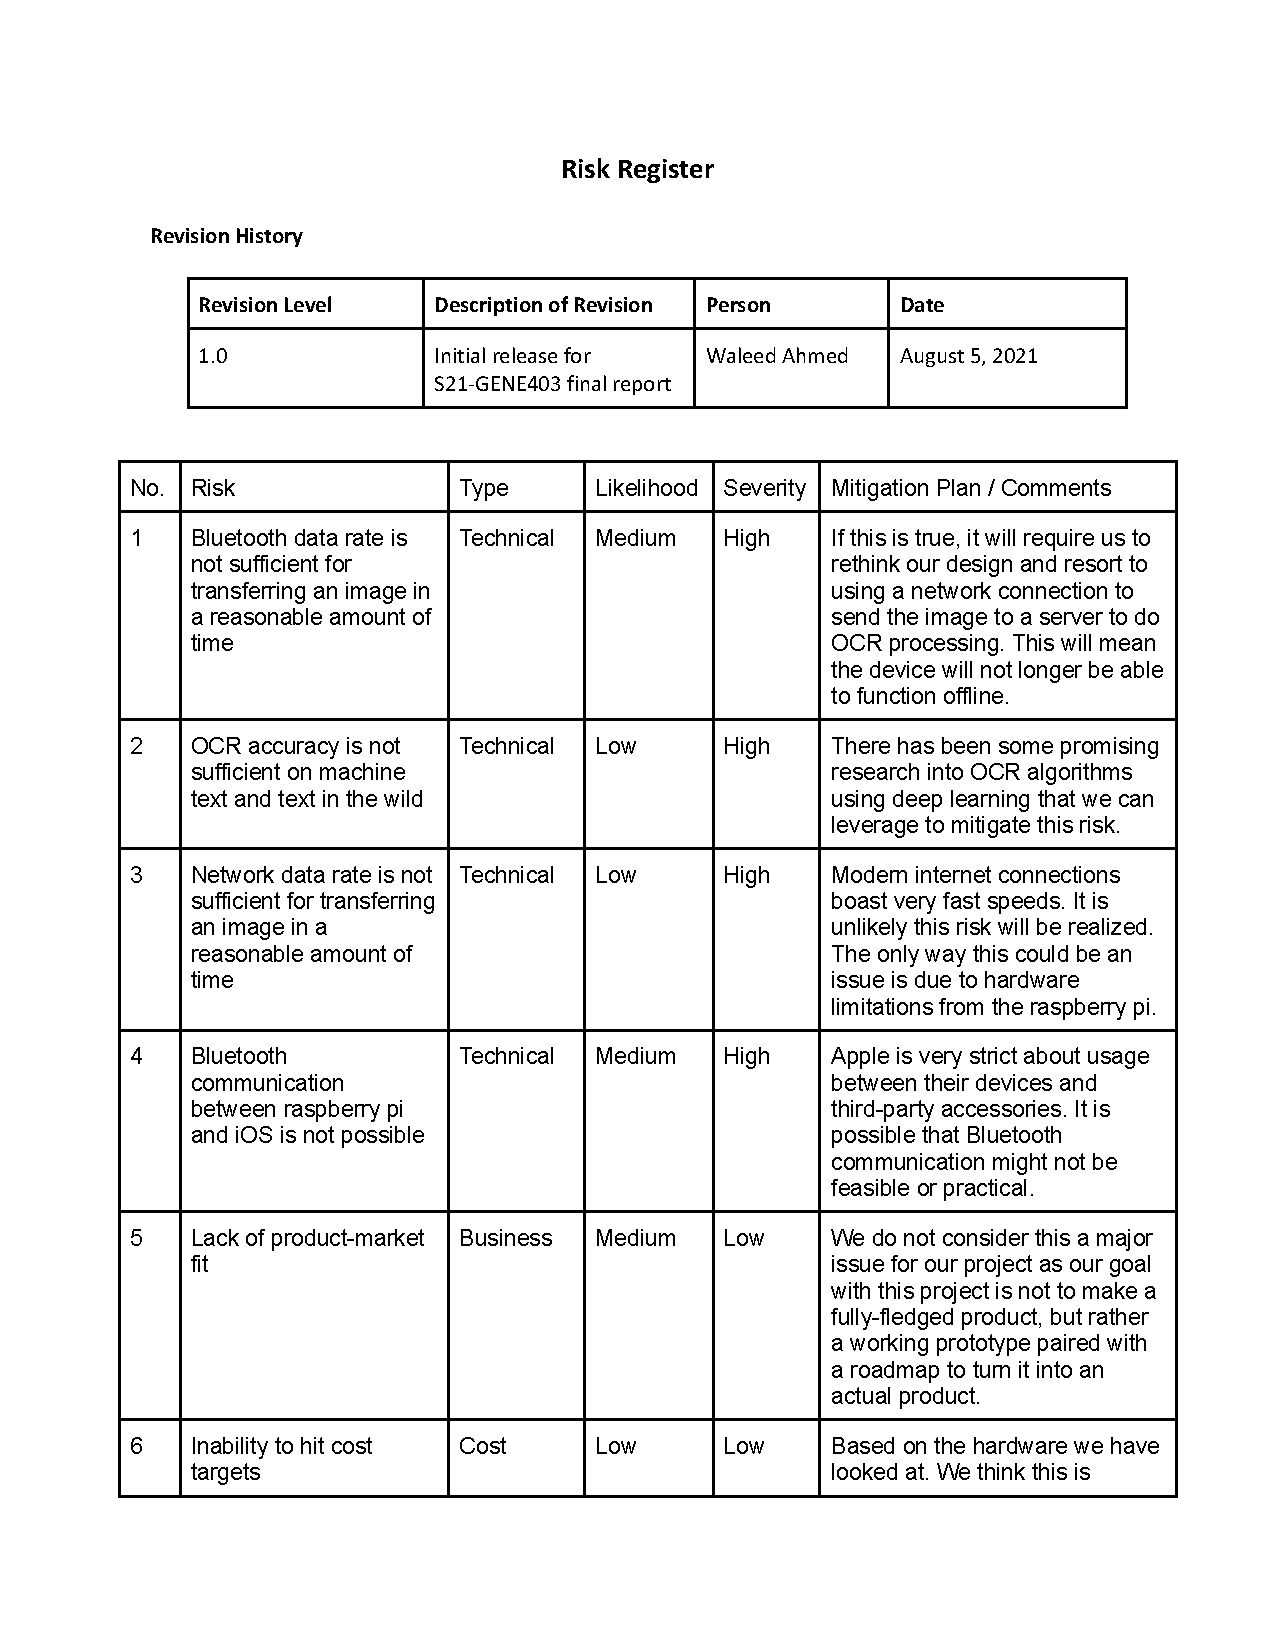
\includegraphics[page=1,width={1.0\linewidth}]{pdf/risk-register-1.0.pdf}
\newpage
\includegraphics[page=2,width={1.0\linewidth}]{pdf/risk-register-1.0.pdf}

\newpage
\subsection{Meeting Logs}
\label{meeting-logs}
Throughout the term, we used a shared Notion drive to hold all meeting logs and research notes.
Below are some screenshots that showcase the organization of the drive and the format we followed for keeping track of meeting logs.

\begin{center}
    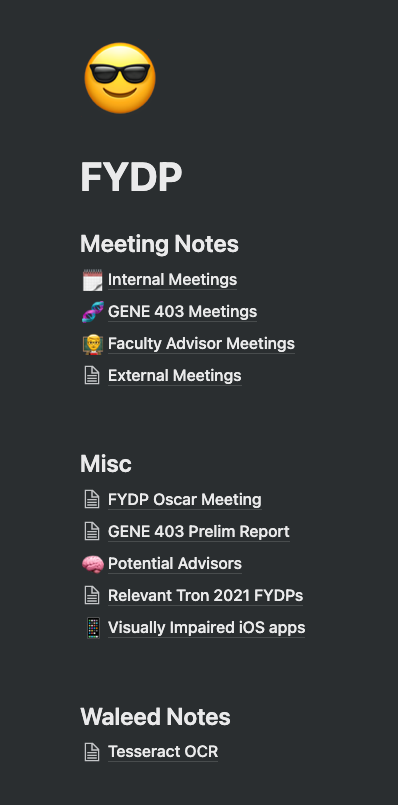
\includegraphics[width={0.3\linewidth}]{img/notion/notion1.png}
    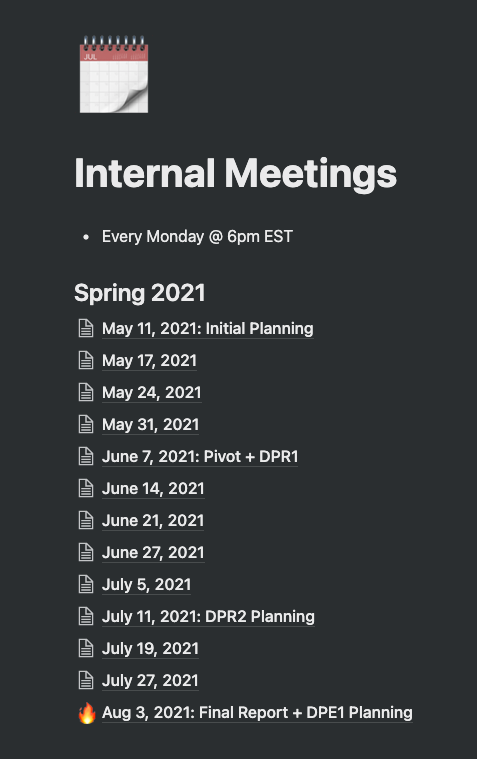
\includegraphics[width={0.35\linewidth}]{img/notion/notion2.png}
    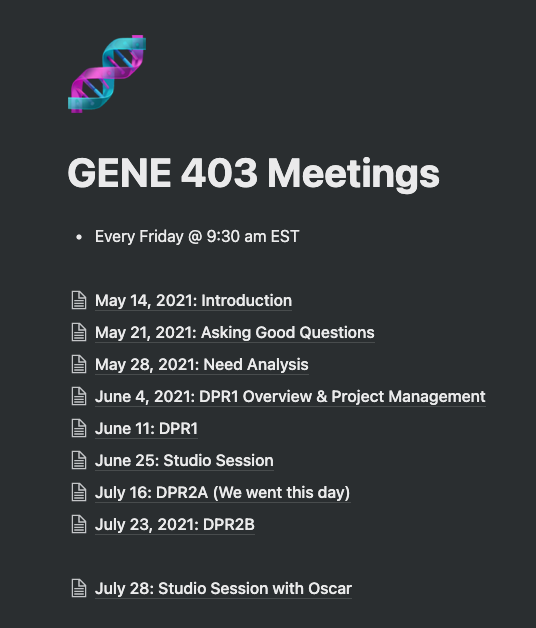
\includegraphics[width={0.3\linewidth}]{img/notion/notion3.png}
    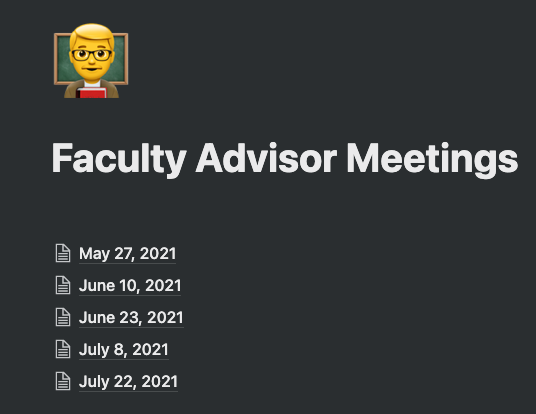
\includegraphics[width={0.3\linewidth}]{img/notion/notion4.png}
    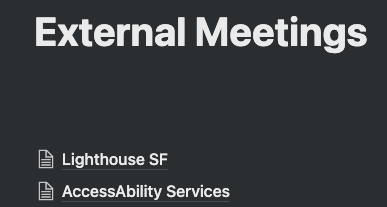
\includegraphics[width={0.3\linewidth}]{img/notion/notion5.png}
\end{center}

\newpage

\noindent
For the internal meeting notes, the format we converged on naturally was:
\begin{itemize}
    \item Updates
        \begin{itemize}
            \item Waleed
            \item Connor
            \item Zain
            \item Martin
        \end{itemize}
    \item Discussion Topics
    \item Action Items
        \begin{itemize}
            \item Waleed
            \item Connor
            \item Zain
            \item Martin
        \end{itemize}
\end{itemize}

\noindent
The idea is for each member to give updates on what they did the previous week, and then we go into any discussion items for that week, and finally end off with each member listing off their current action items. The expectation is that next week's updates will be based on the previous week's action items. An example of our notes from our meeting on August 3rd, 2021 are below:
\begin{center}
    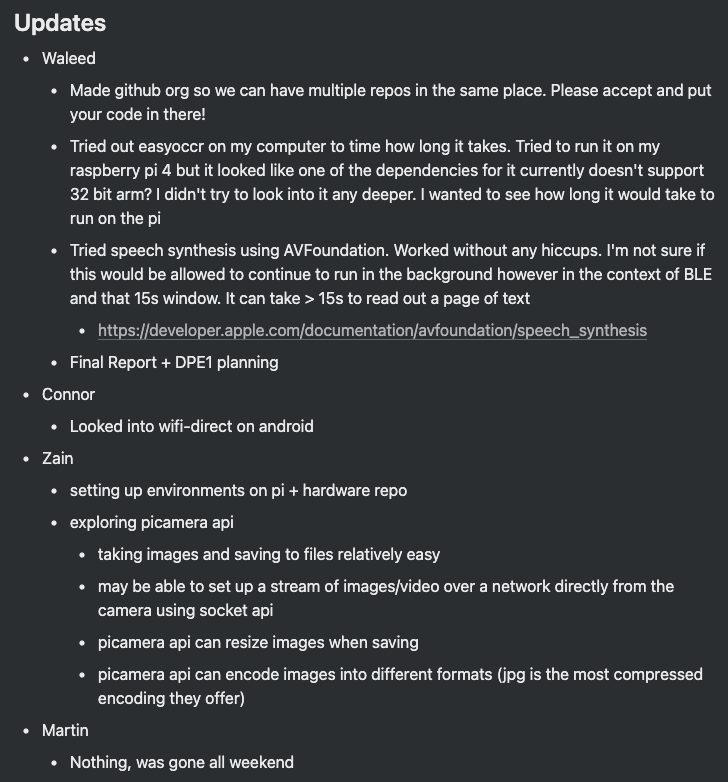
\includegraphics[width={0.5\linewidth}]{img/notion/Aug3_Updates.png} \\
    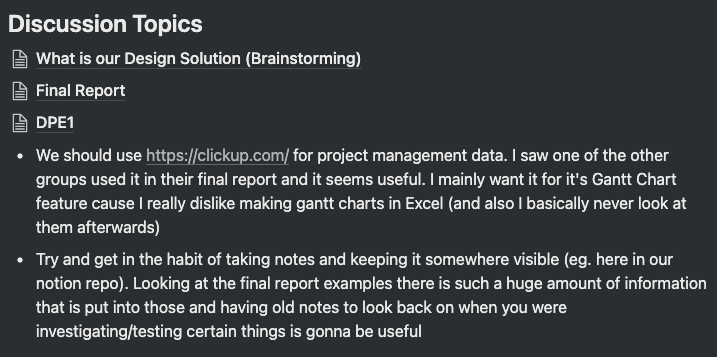
\includegraphics[width={0.45\linewidth}]{img/notion/Aug3_Discussion.png}
    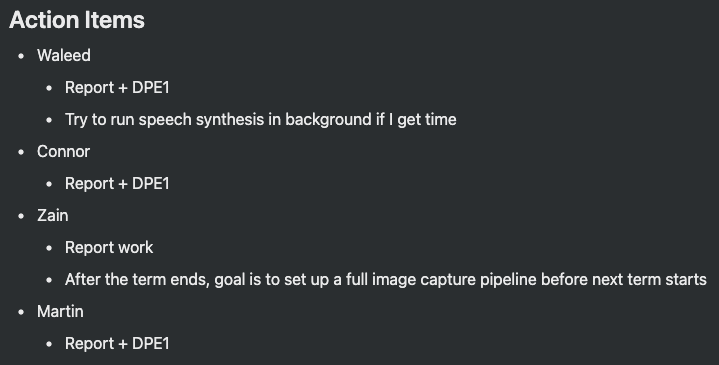
\includegraphics[width={0.45\linewidth}]{img/notion/Aug3_Action.png}
\end{center}

\newpage
\section{Appendix D - Knowledge Application}
\label{appendix-D}
\subsection{OCR Testing Metrics}
Two metrics will be used to evaluate various OCR methods on our custom test sets. For machine text and handwritten text OCR, the word error rate metric is commonly used in the literature \cite{wer-metric}. For text-in-the-wild detection, the F-score metric is commonly used \cite{scene-text-rec}.

\subsubsection{Word Error Rate (WER)}
The Word Error Rate (WER) metric is very similar to the Character Error Rate (CER) metric. However, WER is typically a more useful metric if precise character-level accuracy is not required as long as the meaning of the sentence can be understood, which is the case for most OCR applications.

\

\noindent
Both CER and WER are based on the concept of the Levenshtein Distance. In the context of CER, the Levenshtein Distance corresponds to the minimum number of single-character edits needed to transform one string into another. The allowed character edits are insertion, deletion, and substitution. To apply this to WER, the Levenshtein Distance can be adjusted to be the minimum number of word edits needed to transform a sequence of multiple words to another. \cite{wer-metric}

\

\noindent
The following is an example for displaying the Levenshtein Distance between the words "visual" and "optical". The character edits needed to transform "visual" into "optical" can be seen below:
\begin{enumerate}
  \item \textbf{o}isual: substitute v with o at position 1
  \item o\textbf{p}isual: insert p at position 1
  \item op\textbf{t}isual: insert t at position 1
  \item opti\textbf{c}ual: substitute s with c at position 3
  \item opti\textbf{c}al: delete u at position 4
\end{enumerate}

\noindent
Based on these edits, we can see the Levenshtein Distance is 5. In order to calculate the Levenshtein Distance between two strings, dynamic programming is used. This algorithm will also provide the number of insertions, deletions, and substitutions. These edit counts are what are used in the end to calculate the WER. The dynamic programming algorithm recursively splits the task into smaller tasks of finding the Levenshtein Distance on sub-strings. This generates a DP table. The DP table generated for the example above can be seen in Table \ref{tab:levenshtein_table}. The counts for substitutions, insertions, and deletions can be determined by looking at the number of diagonal, horizontal, and vertical transitions along the highlighted path in the DP table. The final Levenshtein Distance is the value in the bottom-right corner of the table. \cite{levenshtein-dist}

\begin{table}[H]
\begin{center}
\caption{Levenshtein DP table for transforming "visual" to "optical".}
\begin{tabular}{ c|c c c c c c c c } 
  &   & o & p & t & i & c & a & l \\ \hline
  & \textcolor{red}{0} & 1 & 2 & 3 & 4 & 5 & 6 & 7 \\
 v & 1 & \textcolor{red}{1} & \textcolor{red}{2} & \textcolor{red}{3} & 4 & 5 & 6 & 7 \\
 i & 2 & 2 & 2 & 3 & \textcolor{red}{3} & 4 & 5 & 6 \\
 s & 3 & 3 & 3 & 3 & 4 & \textcolor{red}{4} & 5 & 6 \\
 u & 4 & 4 & 4 & 4 & 4 & \textcolor{red}{5} & 5 & 6 \\
 a & 5 & 5 & 5 & 5 & 5 & 5 & \textcolor{red}{5} & 6 \\
 l & 6 & 6 & 6 & 6 & 6 & 6 & 6 & \textcolor{red}{5} \\
\end{tabular}
\label{tab:levenshtein_table}
\end{center}
\end{table}

\noindent
These edit counts can then be fed into Equation \ref{eq:CER} for CER. Where S, D, and I are the number of substitutions, deletions, and insertions respectively and N is the total number of characters in the ground truth string. Note that for Equation \ref{eq:WER}, the counts correspond to full word edits and the denominator is the total number of words in the ground truth text. \cite{wer-metric}

\begin{equation}
\label{eq:CER}
CER=\frac{S+D+I}{N}
\end{equation}

\begin{equation}
\label{eq:WER}
WER=\frac{S_w+D_w+I_w}{N_w}
\end{equation}

\subsubsection{F-Score}
An OCR system typically consists of text detection followed by recognition. In the context of machine text, the difficulty of the detection is negligible. Therefore, a metric that evaluates recognition is only required. However, for text-in-the-wild OCR, the detection task is much more difficult. A metric that takes detection accuracy into account should be used. What is commonly used in research is the F-score metric.

\

\noindent
To calculate the F-score for a given example, counts for true positives (TP), false positives (FP), and false negatives (FN) are needed. A TP in this case is defined as a bounding box prediction which firstly has an intersection over union (IoU) above a certain threshold with any ground truth bounding box and secondly predicts the correct text corresponding to the ground truth. The definition of IoU can be seen in Figure \ref{fig:iou-equation}.

\begin{figure}[H]
\centering
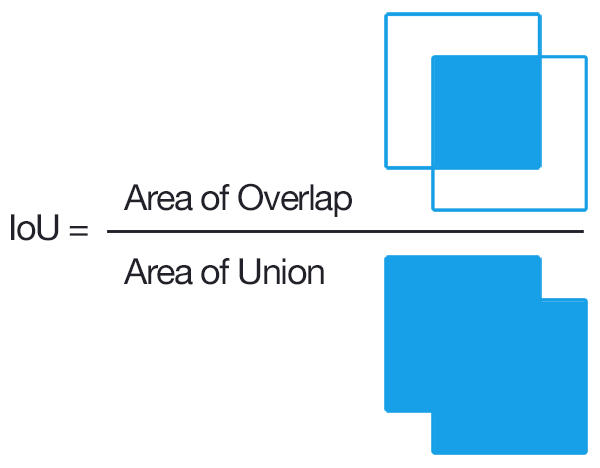
\includegraphics[scale=0.5]{img/iou_equation.png}
\caption{Description of the Intersection over Union (IoU) metric. \cite{iou-object-detection}}
\label{fig:iou-equation}
\end{figure}

\noindent
False positives are then defined as bounding box predictions that do not have an IoU above the desired threshold with any ground truth bounding box or pass the desired IoU but do not provide the correct text prediction. False negatives are defined as any ground truth bounding boxes that do not have any predictions corresponding as true positives with them. As seen in Equations \ref{eq:precision}, \ref{eq:recall}, and \ref{eq:f-score}, these values can then be used to calculate precision (P) and recall (R), which can then be used to calculate the F-score (F) value.

\begin{equation}
\label{eq:precision}
P=\frac{TP}{TP+FP}
\end{equation}

\begin{equation}
\label{eq:recall}
R=\frac{TP}{TP+FN}
\end{equation}

\begin{equation}
\label{eq:f-score}
F=2*\frac{P*R}{P+R}
\end{equation}

\newpage
% REFERENCES
\begin{thebibliography}{9}
\bibitem{orbis-global-blind-data}
“Number of blind people set to triple by 2050” Orbis, 09-Feb-2021. [Online]. Available: https://can.orbis.org/en/news/2017/number-of-blind-people-set-to-triple-by-2050-1. [Accessed: 02-Aug-2021]. 

\bibitem{cnib-blind-data}
“Blindness in Canada” CNIB. [Online]. Available: https://cnib.ca/en/sight-loss-info/blindness/blindness-canada?region=on. [Accessed: 02-Aug-2021]. 

\bibitem{nfb-blind-data}
“Blindness Statistics” NFB, Jan-2019. [Online]. Available: https://nfb.org/resources/blindness-statistics. [Accessed: 02-Aug-2021]. 

\bibitem{lighthouse-sf-info-page}
“What does ‘blind’ really mean?” LightHouse for the Blind and Visually Impaired, 28-Jan-2019. [Online]. Available: https://lighthouse-sf.org/about/getting-started/. [Accessed: 02-Aug-2021]. 

\bibitem{WHO-blindness}
“Vision impairment and blindness” World Health Organization. [Online]. Available: https://www.who.int/news-room/fact-sheets/detail/blindness-and-visual-impairment. [Accessed: 02-Aug-2021]. 

\bibitem{lighthouse-sf-homepage}
LightHouse for the Blind and Visually Impaired, 22-Aug-2019. [Online]. Available: https://lighthouse-sf.org/. [Accessed: 02-Aug-2021].

\bibitem{uw-accessability}
AccessAbility Services, 08-Jul-2021. [Online]. Available: https://uwaterloo.ca/accessability-services/. [Accessed: 03-Aug-2021]. 

\bibitem{jaws-software}
“Jaws®” Freedom Scientific. [Online]. Available: https://www.freedomscientific.com/products/
software/jaws/. [Accessed: 03-Aug-2021].

\bibitem{kurzweil}
K. Education, Assistive learning technologies \& literacy software from KURZWEIL Education. [Online]. Available: https://www.kurzweiledu.com/default.html. [Accessed: 03-Aug-2021]. 

\bibitem{read-and-write}
“Read \& write for education - reading, literacy \& assistive software” Texthelp. [Online]. Available: https://www.texthelp.com/en-gb/products/read-and-write-education/. [Accessed: 03-Aug-2021]. 

\bibitem{speechify}
Speechify. [Online]. Available: https://speechify.com/. [Accessed: 03-Aug-2021]. 

\bibitem{clickup}
“ClickUp™ | one app to replace them all.” [Online]. Available: https://clickup.com/. [Accessed: 07-Aug-2021]. 

\bibitem{orcam}
OrCam MyEye 2.0. [Online]. Available: https://www.orcam.com/en/myeye2/. [Accessed: 08-Aug-2021].

\bibitem{orcam-price}
B. Holton, “MyReader and MyEye from OrCam: Text and item recognition at the touch of a finger,” The American Foundation for the Blind. [Online]. Available: https://www.afb.org/aw/18/2/15244. [Accessed: 08-Aug-2021]. 

\bibitem{orcam-amazon}
“OrCam MyEye Pro ,” Amazon.ca: Electronics. [Online]. Available: https://www.amazon.ca/OrCam-Inc-MyEye-2/dp/B07H31SBMW. [Accessed: 08-Aug-2021].

\bibitem{WHO-assistive}
“Assistive technology,” World Health Organization. [Online]. Available: https://www.who.int/news-room/fact-sheets/detail/assistive-technology. [Accessed: 08-Aug-2021]. 

\bibitem{envision}
Envision. [Online]. Available: https://www.letsenvision.com/. [Accessed: 08-Aug-2021].

\bibitem{seeing-ai}
Seeing AI App from Microsoft. [Online]. Available: https://www.microsoft.com/en-us/ai/seeing-ai. [Accessed: 08-Aug-2021]. 

\bibitem{speechify}
Speechify. [Online]. Available: https://speechify.com/. [Accessed: 08-Aug-2021]. 

\bibitem{be-my-eyes}
Be My Eyes - See the world together. [Online]. Available: https://www.bemyeyes.com/. [Accessed: 08-Aug-2021]. 

\bibitem{tesseract-github}
“Tesseract-Ocr/Tesseract: Tesseract open source ocr engine (main repository),” GitHub. [Online]. Available: https://github.com/tesseract-ocr/tesseract. [Accessed: 09-Aug-2021]. 

\bibitem{apple-speech-synthesis}
“Speech Synthesis,” Apple Developer Documentation. [Online]. Available: https://developer.apple.com/documentation/avfoundation/speech\_synthesis. [Accessed: 09-Aug-2021]. 

\bibitem{tesseract-improve-quality}
“Improving the quality of the output,” tessdoc. [Online]. Available: https://tesseract-ocr.github.io/tessdoc/ImproveQuality.html. [Accessed: 09-Aug-2021]. 

\bibitem{apple-mfi}
“Create innovative Accessories,” MFi Program. [Online]. Available: https://mfi.apple.com/. [Accessed: 10-Aug-2021]. 

\bibitem{apple-wac}
“Wireless Accessory Configuration Entitlement,” Apple Developer Documentation. [Online]. Available: https://developer.apple.com/documentation/bundleresources/entitlements/com\_apple\_external-accessory\_wireless-configuration. [Accessed: 10-Aug-2021]. 

\bibitem{rpi-zero-w}
“Raspberry Pi Zero W,” Raspberry Pi. [Online]. Available: https://www.raspberrypi.org/products/raspberry-pi-zero-w/. [Accessed: 10-Aug-2021]. 

\bibitem{rpi-camera}
“Camera Module 2,” Raspberry Pi. [Online]. Available: https://www.raspberrypi.org/products/camera-module-v2/. [Accessed: 10-Aug-2021]. 

\bibitem{wer-metric}
K. Leung, “Evaluate ocr output quality with character error rate (cer) and word error rate (wer),” Medium, 27-Jul-2021. [Online]. Available: https://towardsdatascience.com/evaluating-ocr-output-quality-with-character-error-rate-cer-and-word-error-rate-wer-853175297510. [Accessed: 10-Aug-2021].

\bibitem{levenshtein-dist}
“Levenshtein distance,” Wikipedia, 09-Mar-2021. [Online]. Available: https://en.wikipedia.org/wiki/Levenshtein\_distance. [Accessed: 10-Aug-2021].

\bibitem{scene-text-rec}
Y. Cao, S. Ma, and H. Pan, “FDTA: Fully CONVOLUTIONAL Scene text detection with TEXT ATTENTION,” IEEE Access, vol. 8, pp. 155441–155449, 2020.

\bibitem{iou-object-detection}
A. Rosebrock, “Intersection over Union (iou) for object detection,” PyImageSearch, 01-Jul-2021. [Online]. Available: https://www.pyimagesearch.com/2016/11/07/intersection-over-union-iou-for-object-detection. [Accessed: 10-Aug-2021].

\bibitem{paddle-ocr}
PaddlePaddle, “PaddlePaddle/PaddleOCR: Awesome Multilingual OCR toolkits based on PaddlePaddle (practical ultra lightweight OCR system, support 80+ Languages recognition, provide data annotation and synthesis tools, support training and deployment among server, mobile, embedded and Iot devices),” GitHub. [Online]. Available: https://github.com/PaddlePaddle/PaddleOCR. [Accessed: 10-Aug-2021].

\bibitem{easy-ocr}
JaidedAI, “JaidedAI/EasyOCR: Ready-to-use OCR with 80+ supported languages and all popular writing scripts including Latin, Chinese, Arabic, Devanagari, Cyrillic and etc.,” GitHub. [Online]. Available: https://github.com/JaidedAI/EasyOCR. [Accessed: 10-Aug-2021].

\bibitem{orcam-patents}
https://www.orcam.com/en/patents/

\bibitem{envision-patent}
https://patents.google.com/patent/US9805619B2/en

\bibitem{orcam-hardware}
https://patents.google.com/patent/US8902303B2/en

\bibitem{orcam-software}
https://patents.justia.com/patent/9911361

\bibitem{doctrine-of-equivalents}
“Doctrine of Equivalents”, Wikipedia, 02-Jun-2021. [Online]. Available: https://en.wikipedia.org/wiki/Doctrine\_of\_equivalents. [Accessed: 09-Aug-2021].

\bibitem{pipeda}
https://www.priv.gc.ca/en/privacy-topics/privacy-laws-in-canada/the-personal-information-protection-and-electronic-documents-act-pipeda/pipeda\_brief/

\bibitem{ewaste}
"What Are The Right Electronic Waste Disposal Methods?", Dawn DeVroom, 30-Apr-2019. [Online]. Available: https://blog.idrenvironmental.com/what-are-the-right-electronic-waste-disposal-methods. [Accessed: 9-Aug-2021]

\bibitem{neural-efficiency}
“Apple A11”, Wikipedia, 02-Jun-2021. [Online]. Available:
https://en.wikipedia.org/wiki/Apple\_A11. [Accessed: 9-Aug-2021].

\bibitem{iphone-recycle}
https://www.apple.com/ca/environment/

\bibitem{apple-bluetooth}
“Core Bluetooth”, Apple Developer Documentation. [Online]. Available: https://developer.apple.com/documentation/corebluetooth. [Accessed: 09-Aug-2021]. 

\bibitem{raspi-hardware}
https://www.raspberrypi.org/products/raspberry-pi-zero-w/

\bibitem{iphone-hardware}
“iPhone X Specifications”, Apple. [Online]. Available: https://support.apple.com/kb/sp770?locale=en\_CA. [Accessed: 09-Aug-2021]. 

\bibitem{bluetooth-classic}
"Bluetooth Classic vs Bluetooth Low Energy (BLE) on Android", D. Kliszowki, A. Vlasov. [Online]. Available: https://www.thedroidsonroids.com/blog/bluetooth-classic-vs-bluetooth-low-energy-ble. [Accessed: 09-Aug-2021].


\end{thebibliography}

\end{document}
